\section{Angular acceptance}
\label{app:Efficiencies}

In this section are reported plots of angular acceptances as a function of $\cos\theta_\ell$ in bins of $\cos\theta_\Lambda$
and viceversa, in different bins of \qsq. 2D plots of efficiency as a function of $\cos\theta_\ell$ versus $\cos\theta_\Lambda$
are also reported.


\begin{figure}[h!]
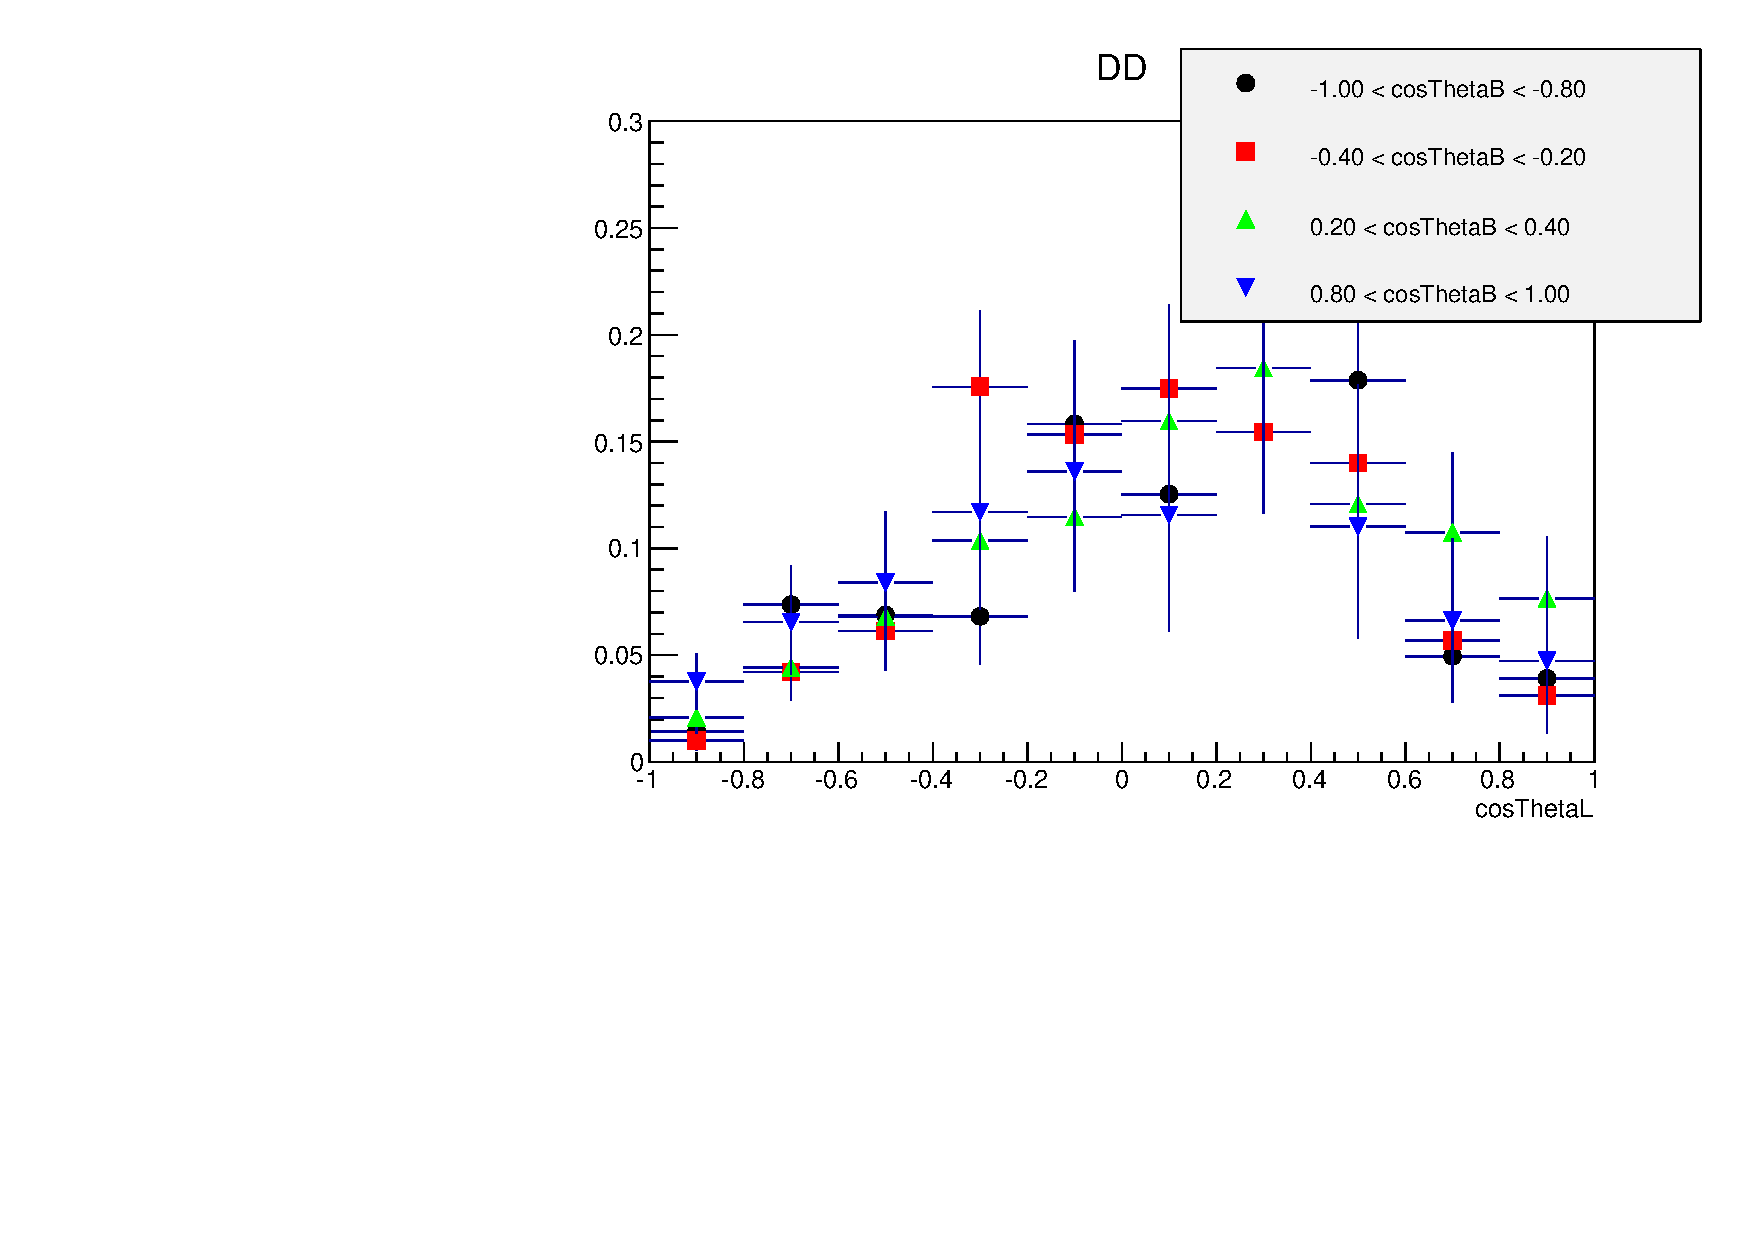
\includegraphics[width=0.45\textwidth]{Lmumu/figs/effs/DDeff_lowestq2.pdf}
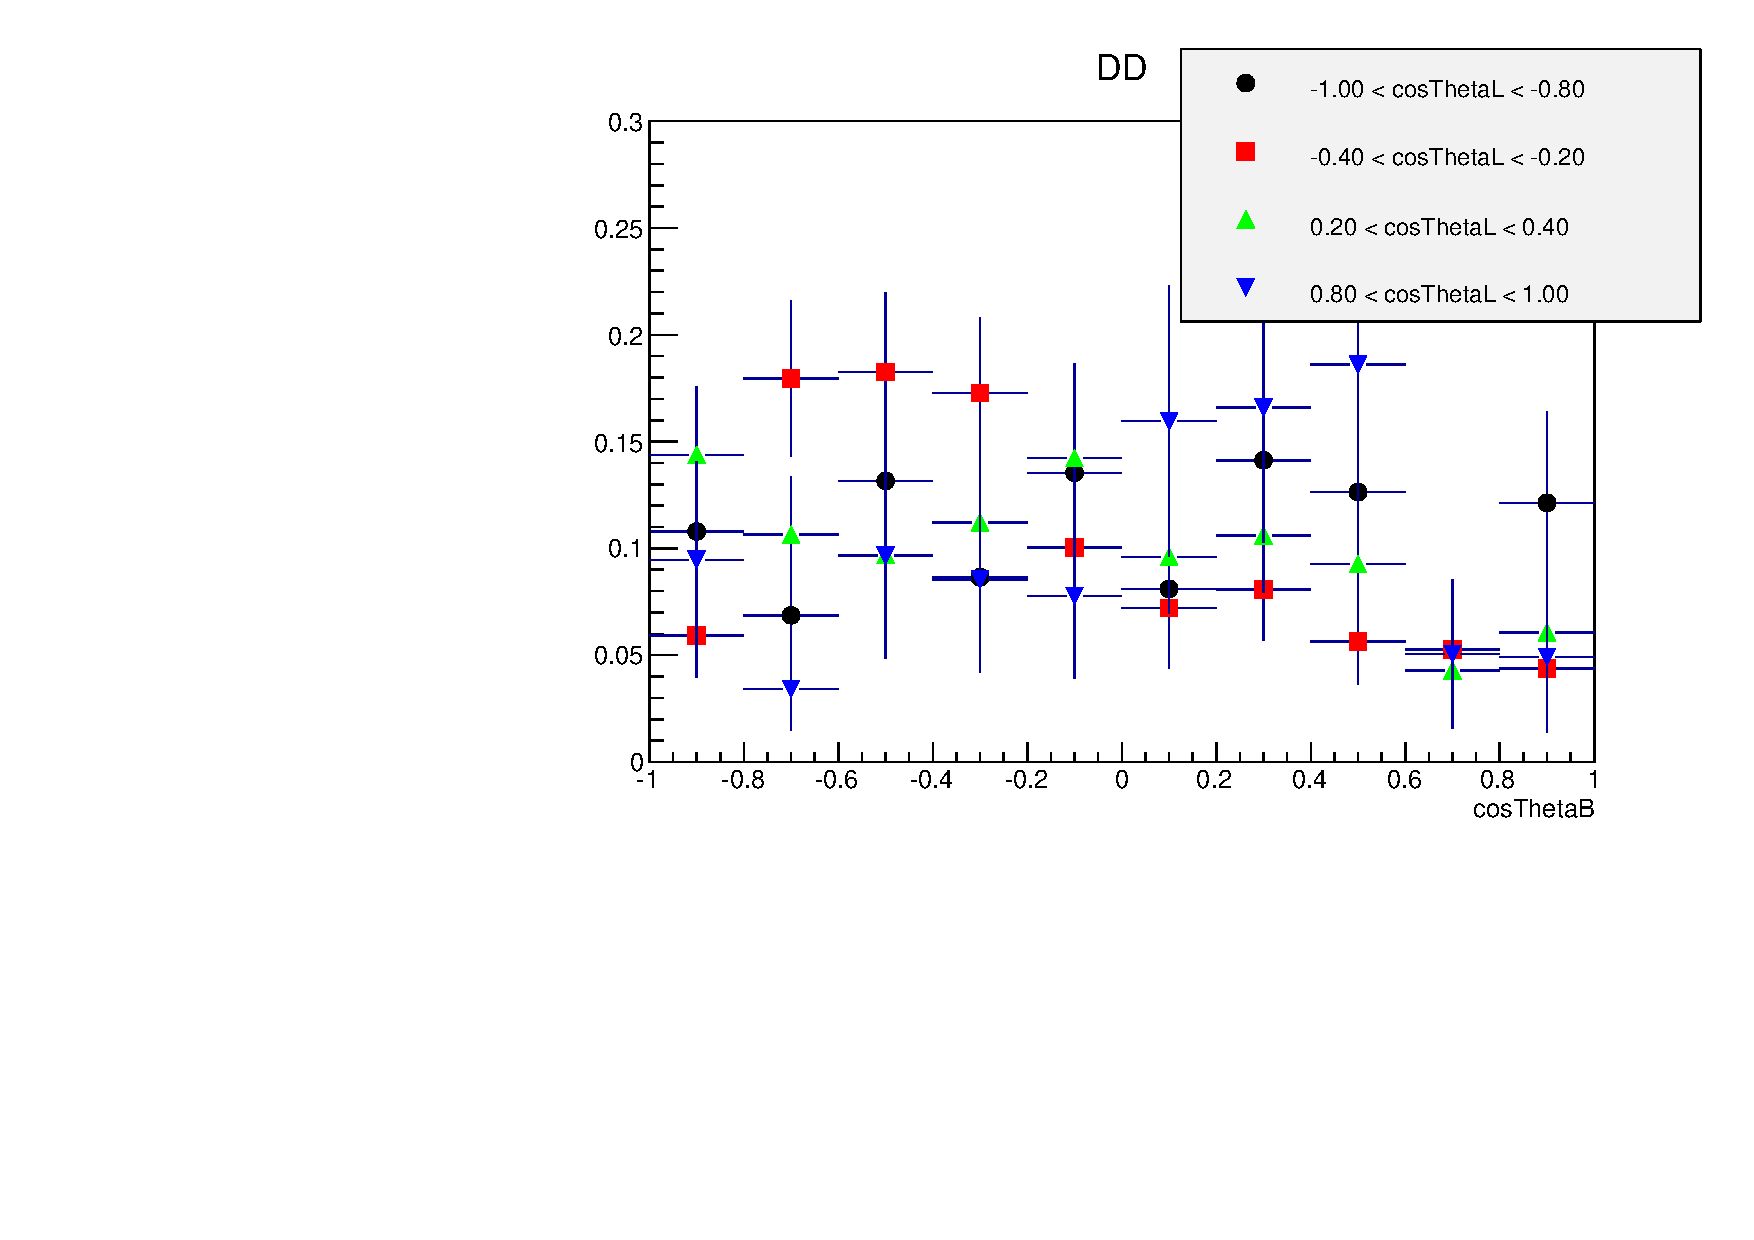
\includegraphics[width=0.45\textwidth]{Lmumu/figs/effs/DDBeff_lowestq2.pdf} 
\caption{Angular acceptance as a function of $\cos\theta_\ell$ in bins of $\cos\theta_\Lambda$ (left) and viceversa (right). For down-down events in the lowest \qsq bin: $1.1 < q^2 < 3$}
\end{figure}


\begin{figure}[h!]
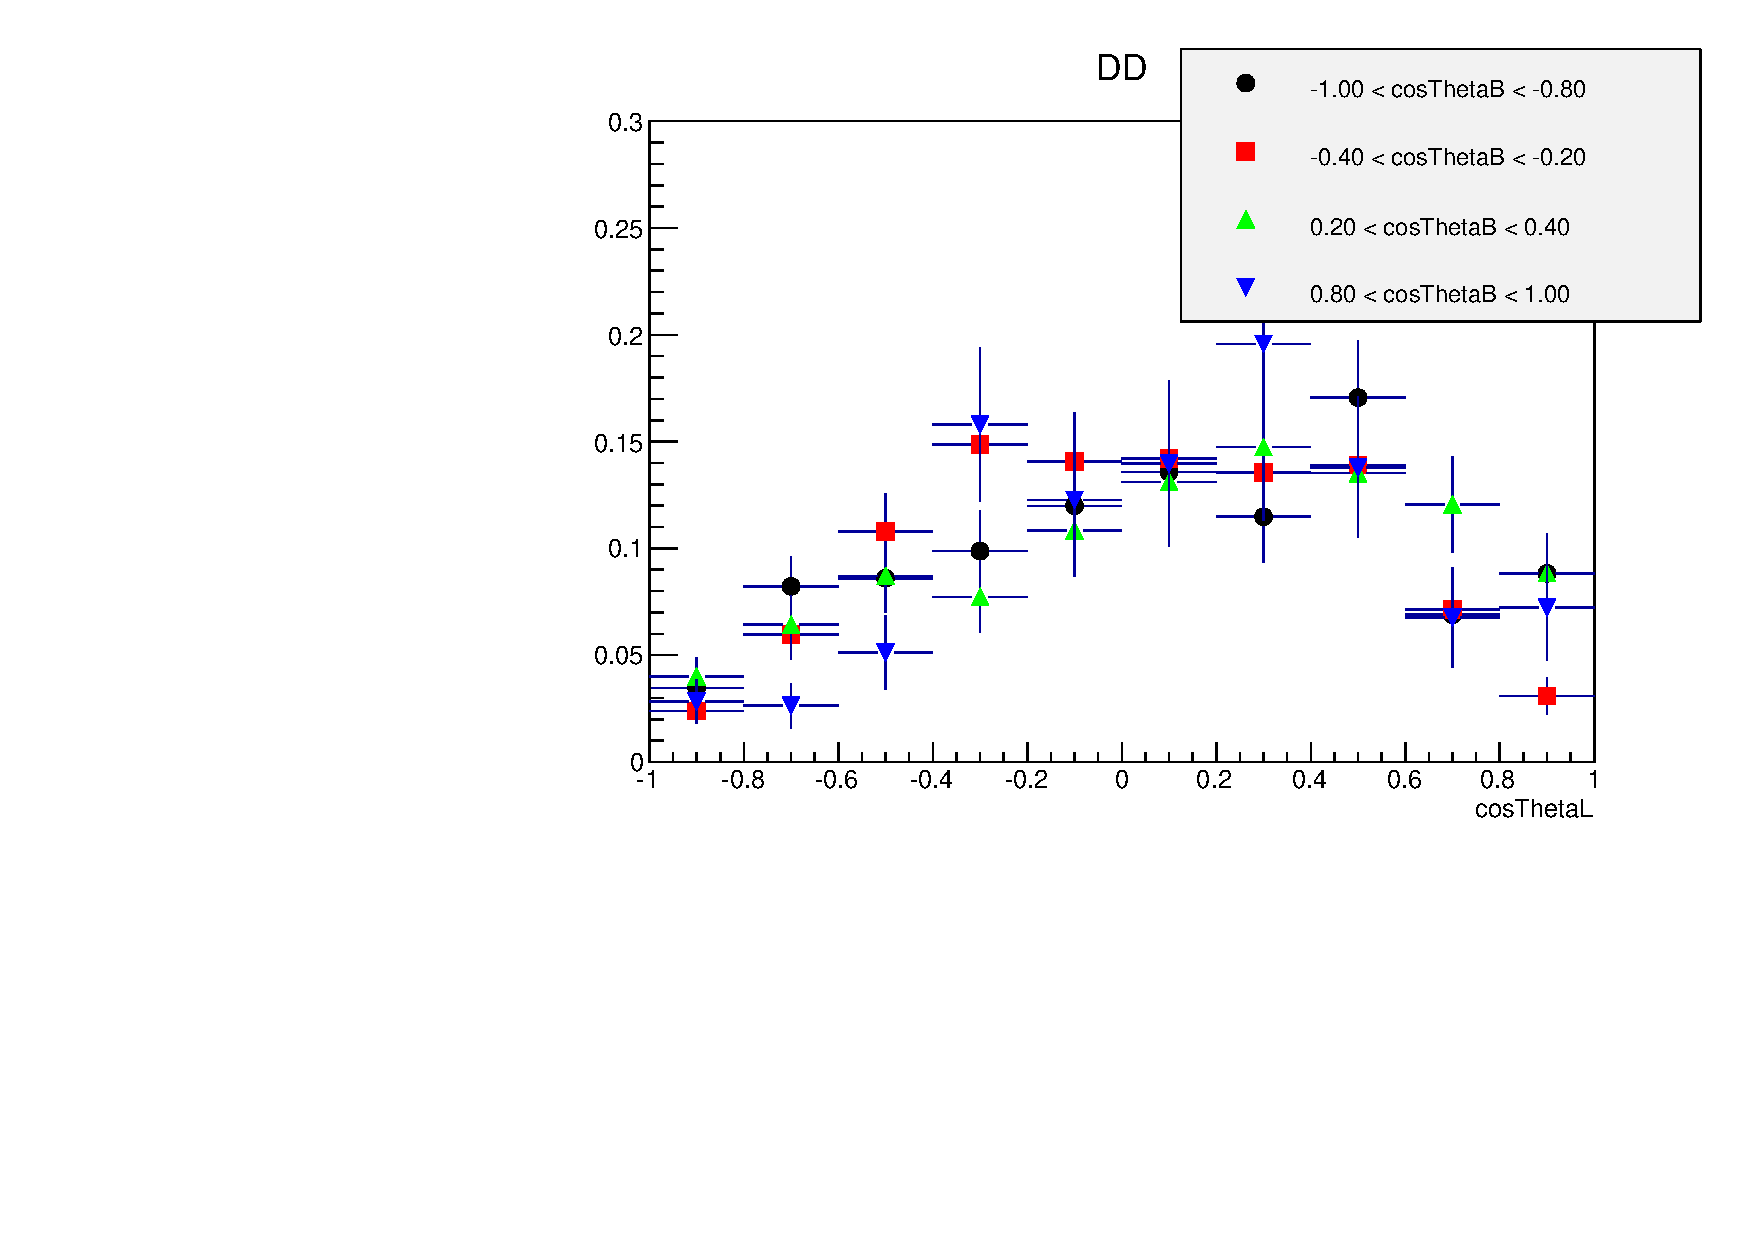
\includegraphics[width=0.45\textwidth]{Lmumu/figs/effs/DDeff_lowq2.pdf}
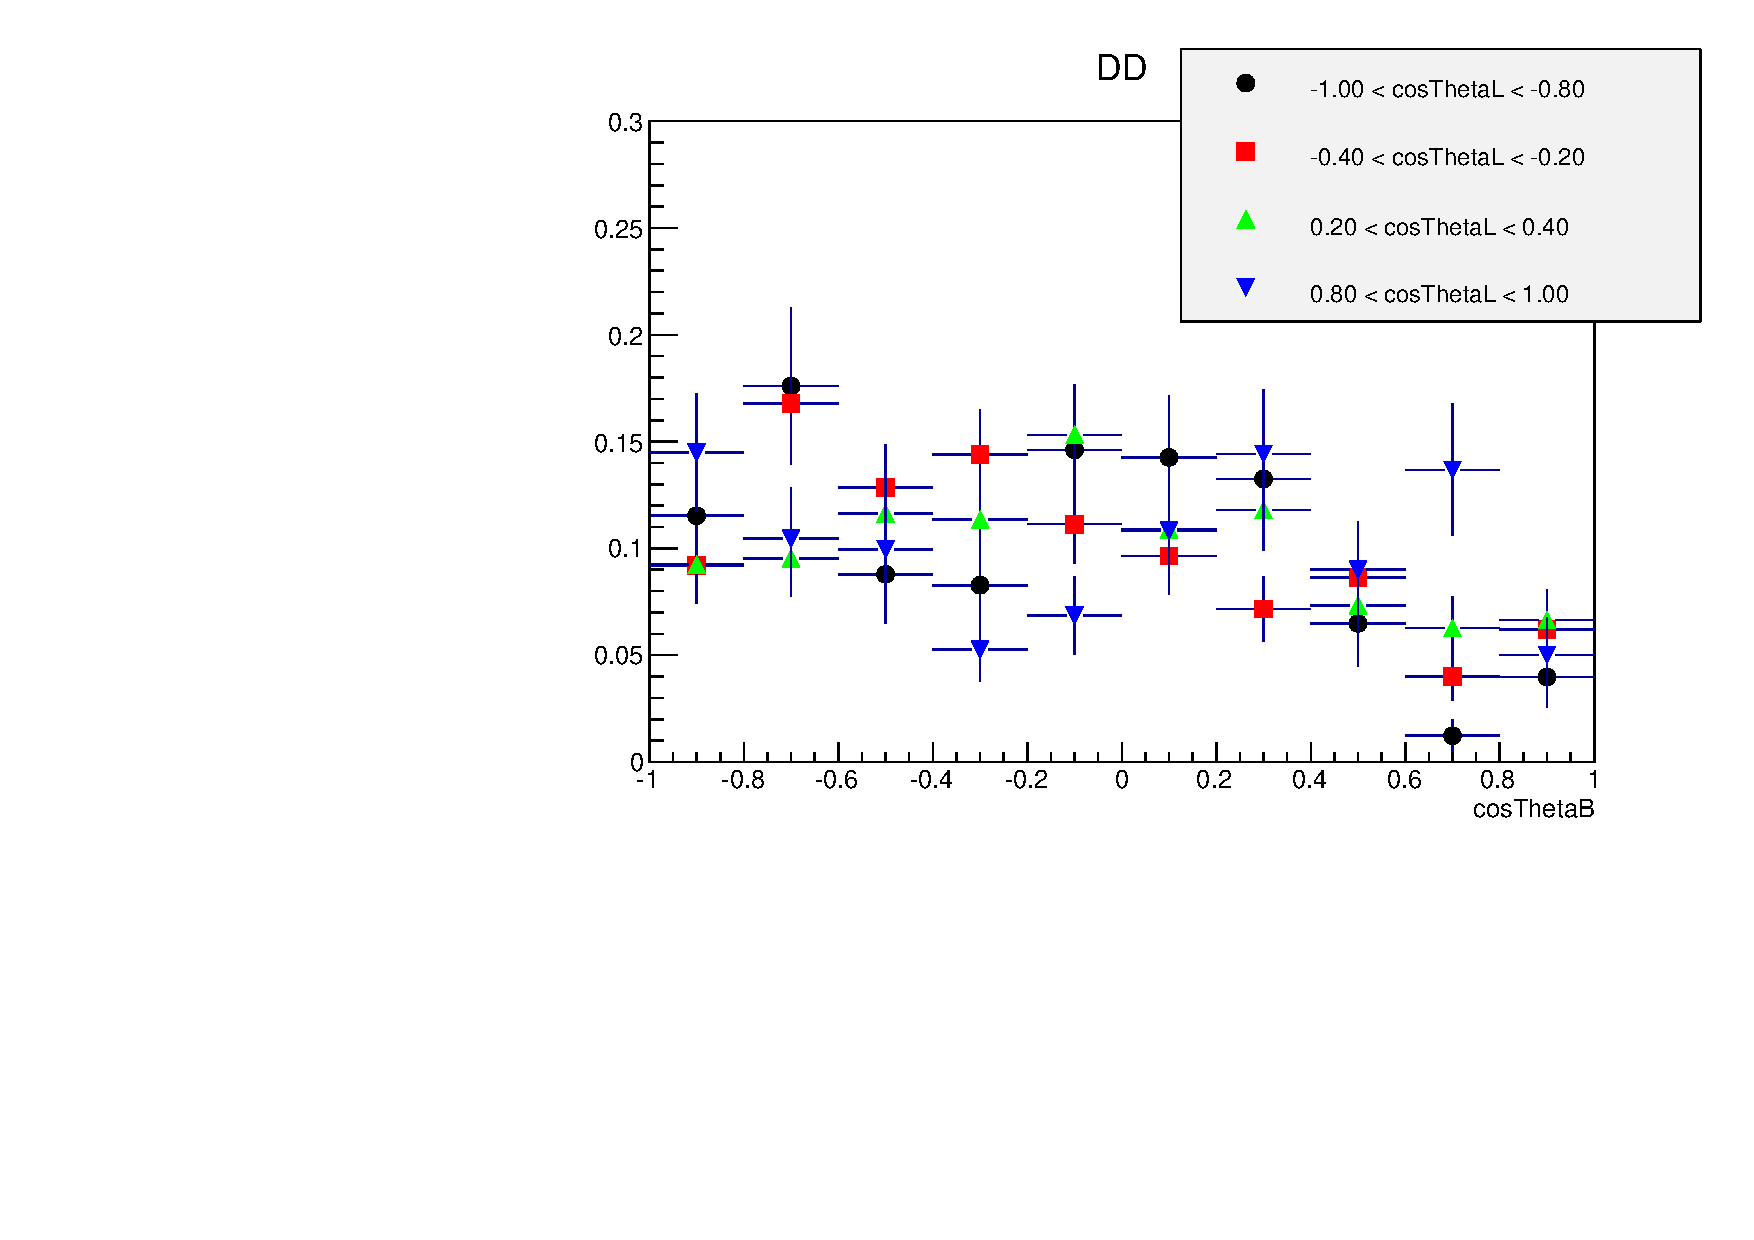
\includegraphics[width=0.45\textwidth]{Lmumu/figs/effs/DDBeff_lowq2.pdf} 
\caption{Angular acceptance as a function of $\cos\theta_\ell$ in bins of $\cos\theta_\Lambda$ (left) and viceversa (right). For down-down events in the integrated low \qsq bin: $1.1 < q^2 < 6$}
\end{figure}

\begin{figure}[h!]
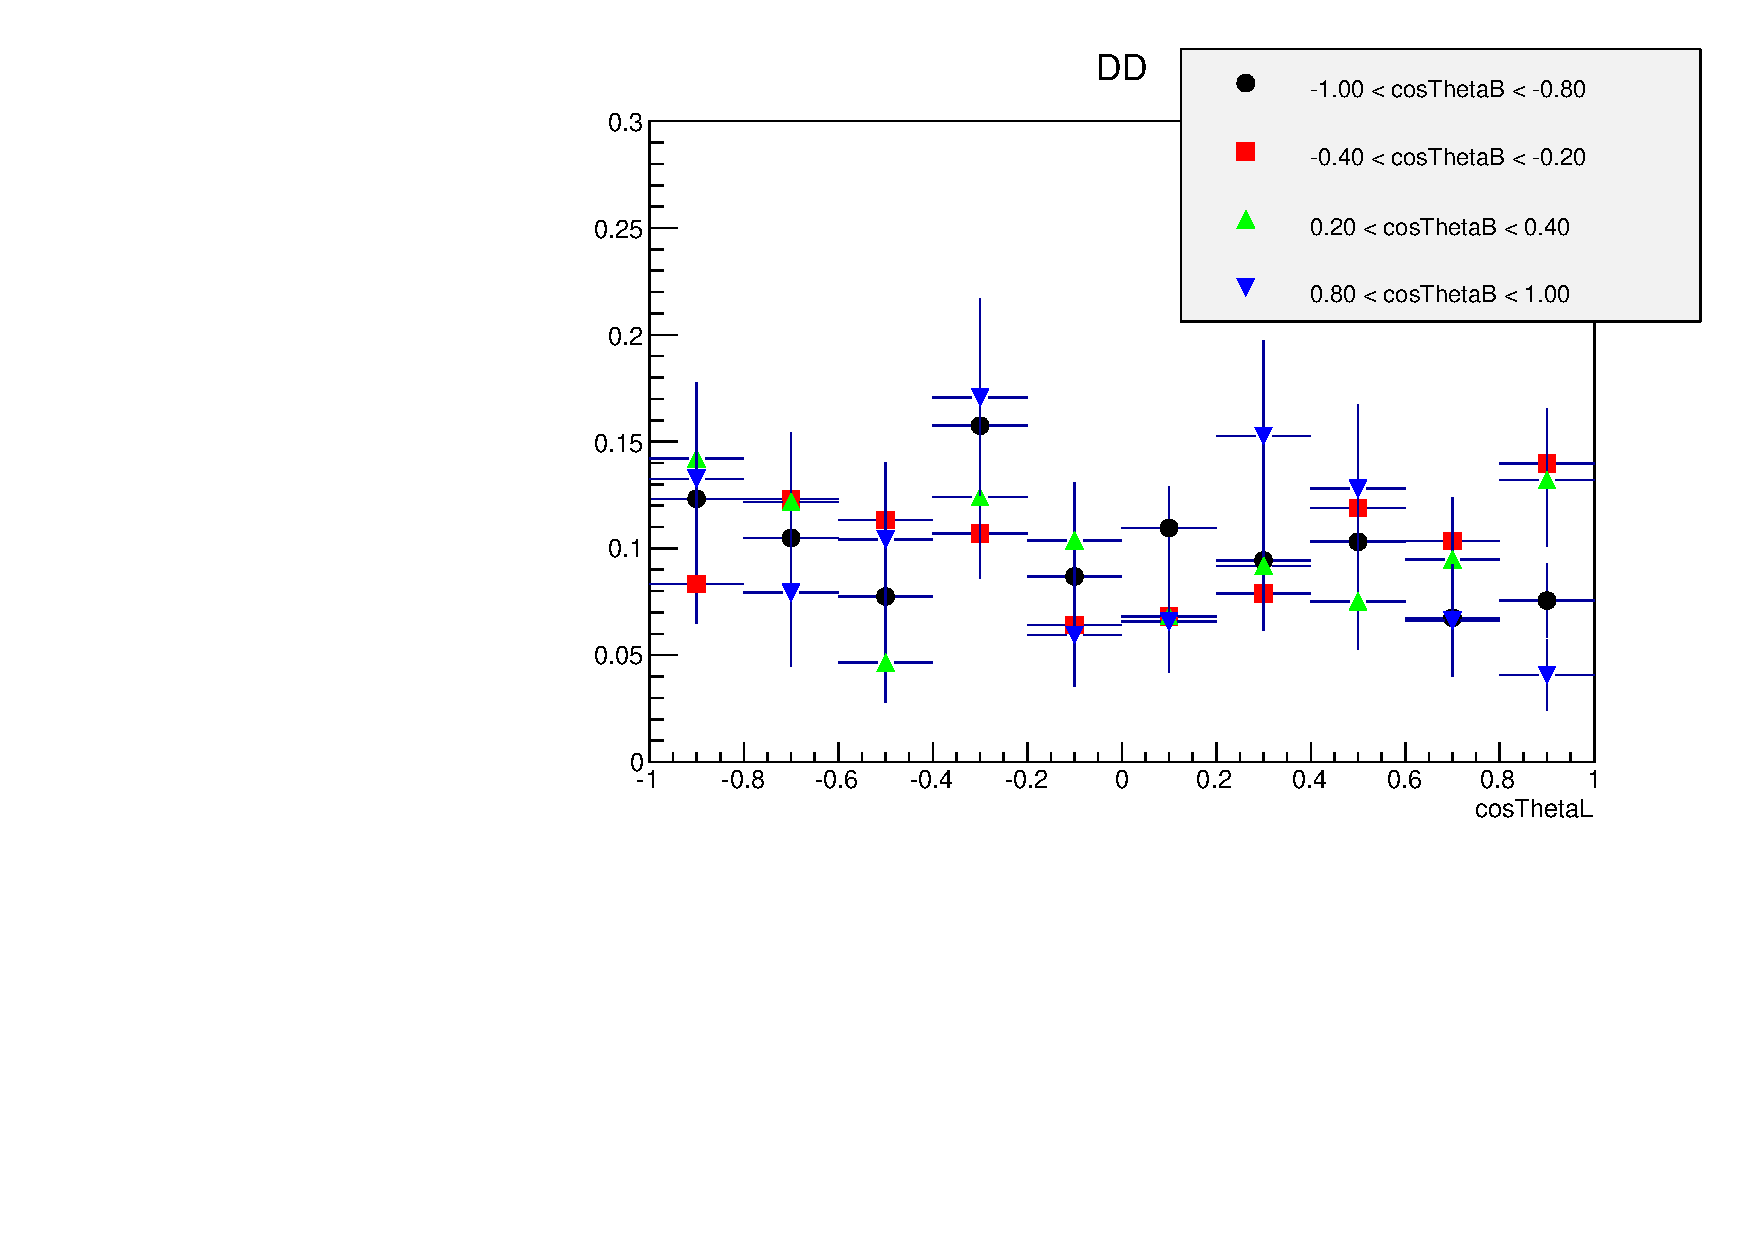
\includegraphics[width=0.45\textwidth]{Lmumu/figs/effs/DDeff_highq2.pdf}
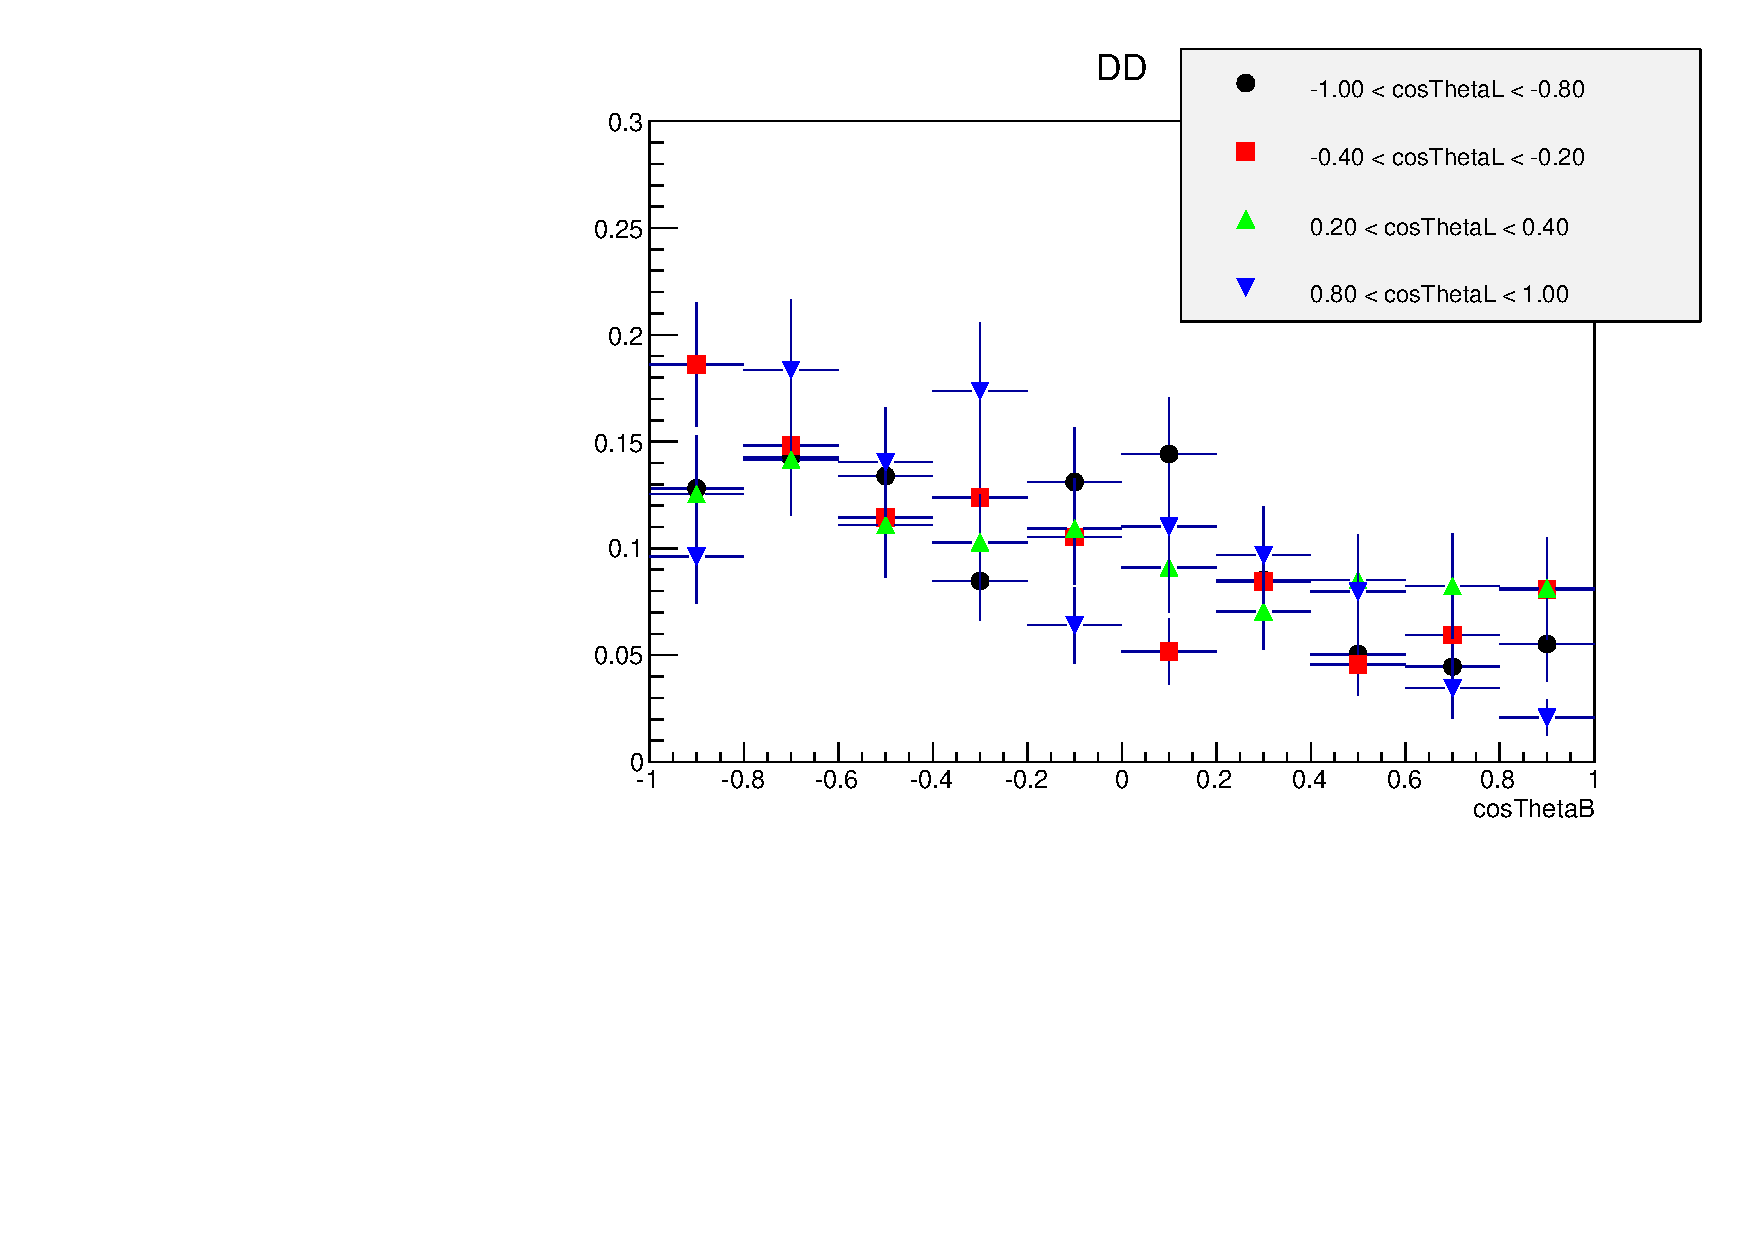
\includegraphics[width=0.45\textwidth]{Lmumu/figs/effs/DDBeff_highq2.pdf} 
\caption{Angular acceptance as a function of $\cos\theta_\ell$ in bins of $\cos\theta_\Lambda$ (left) and viceversa (right). For down-down events in the integrated high \qsq bin: $15 < q^2 < 20$}
\end{figure}

\begin{figure}[h!]
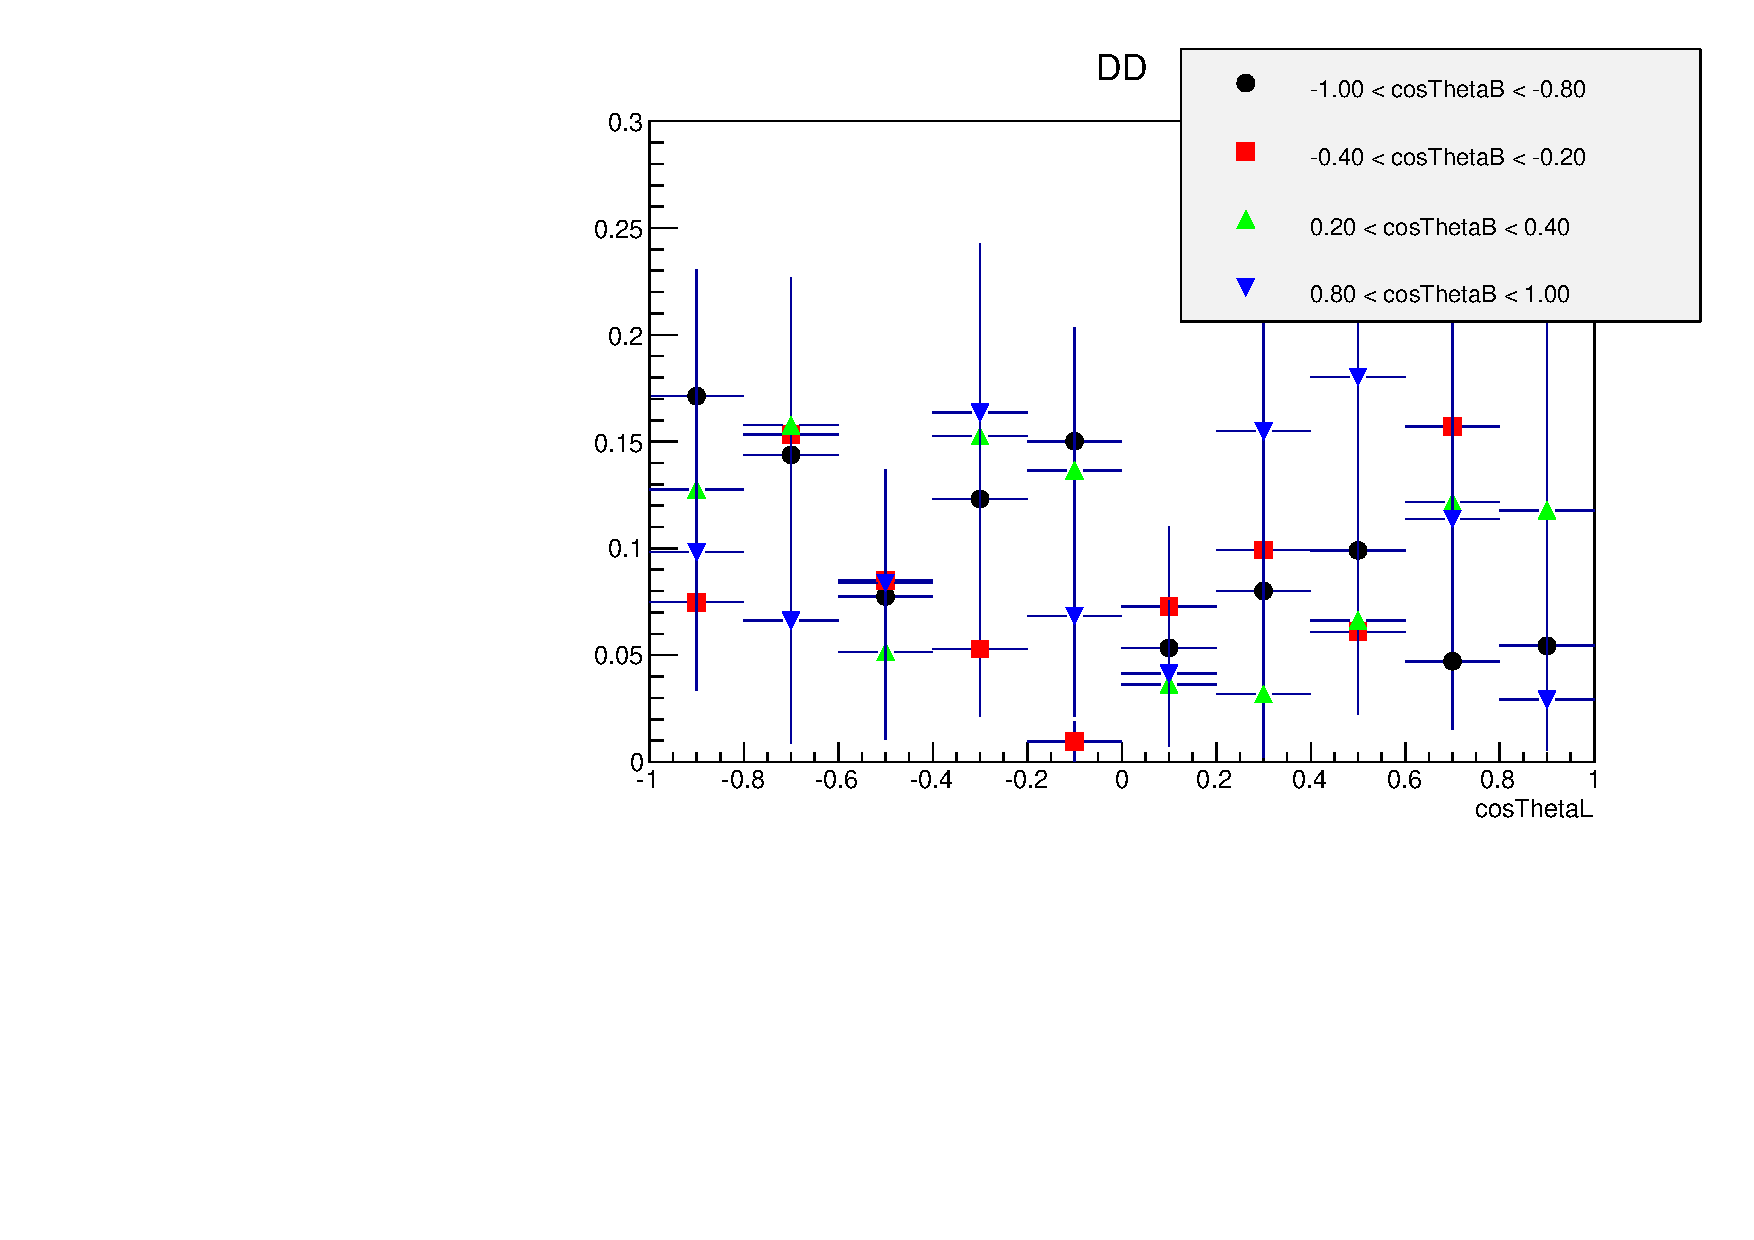
\includegraphics[width=0.45\textwidth]{Lmumu/figs/effs/DDeff_highestq2.pdf}
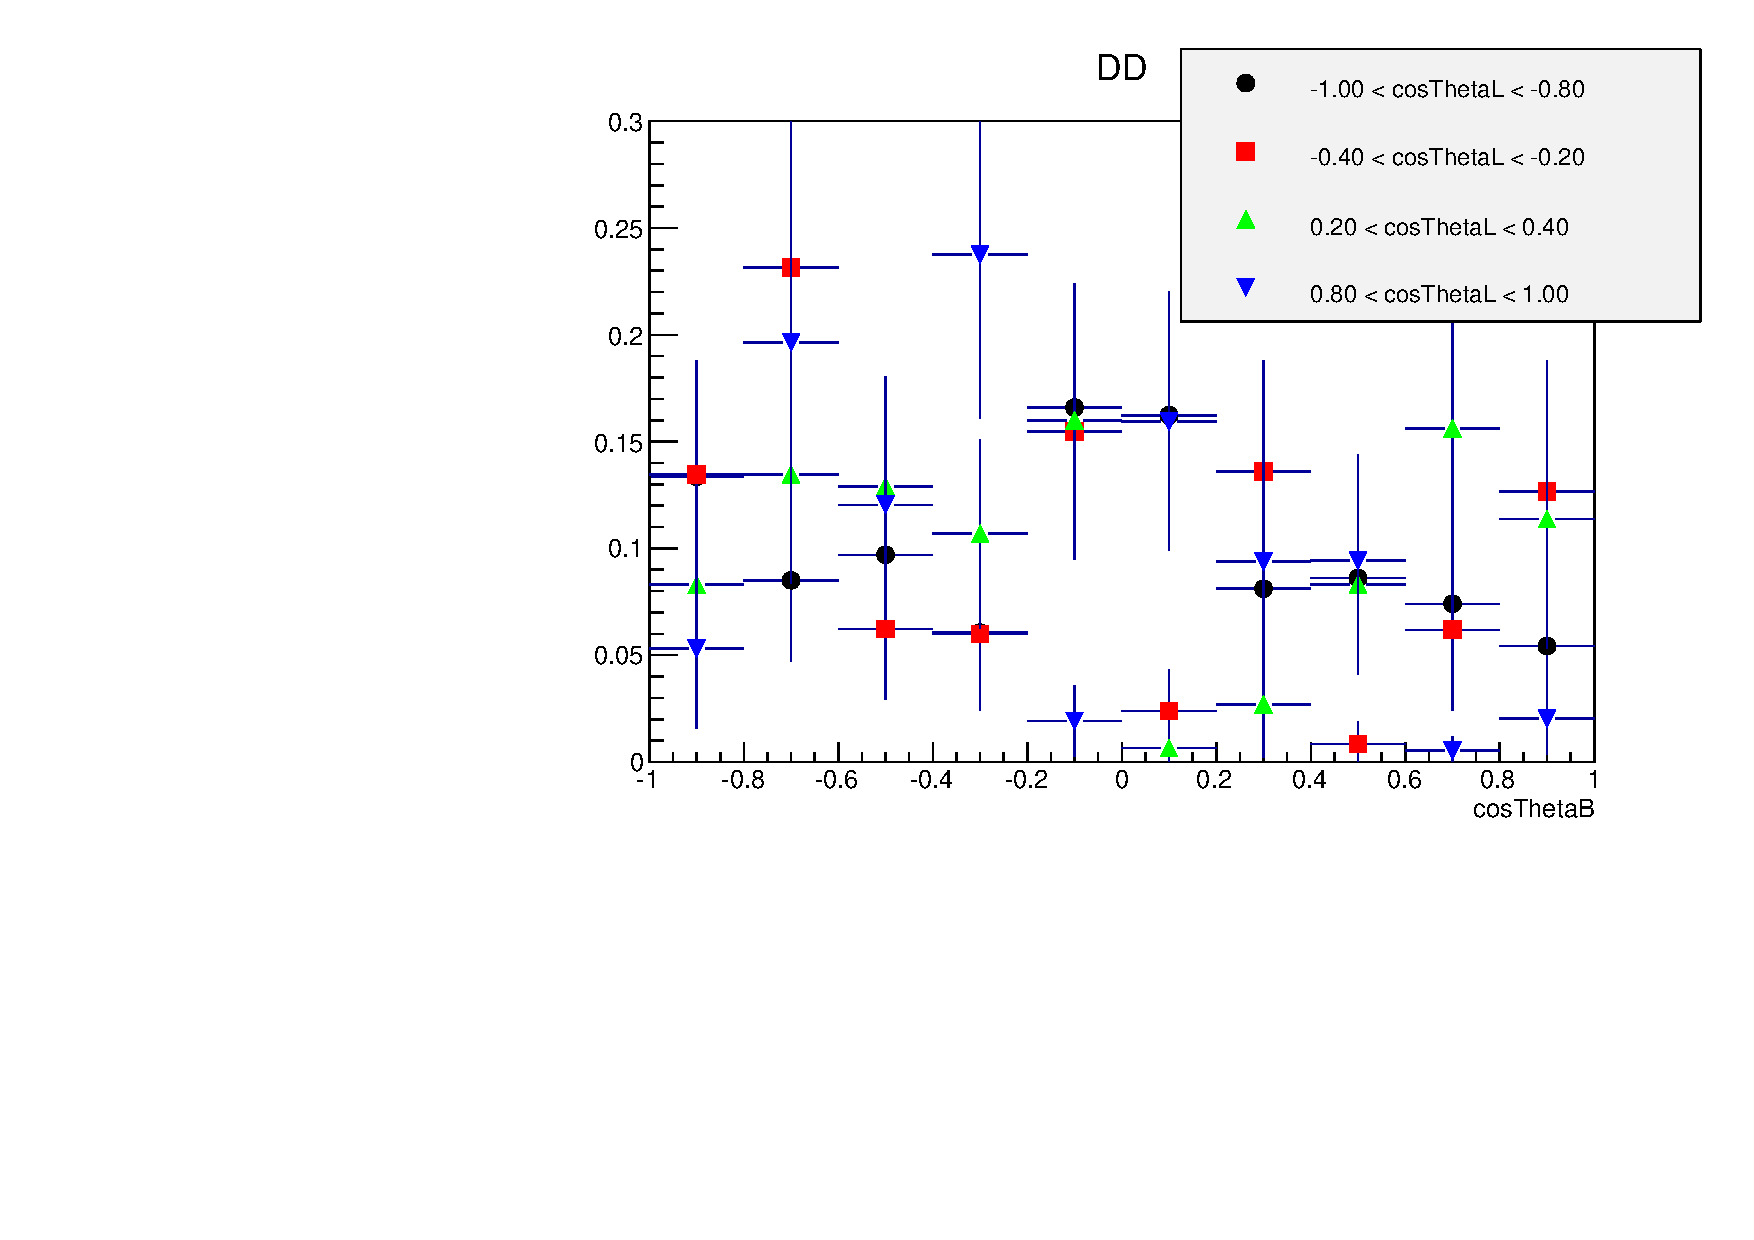
\includegraphics[width=0.45\textwidth]{Lmumu/figs/effs/DDBeff_highestq2.pdf} 
\caption{Angular acceptance as a function of $\cos\theta_\ell$ in bins of $\cos\theta_\Lambda$ (left) and viceversa (right). For down-down events in the highest \qsq bin: $18 < q^2 < 20$}
\end{figure}



\begin{figure}[h!]
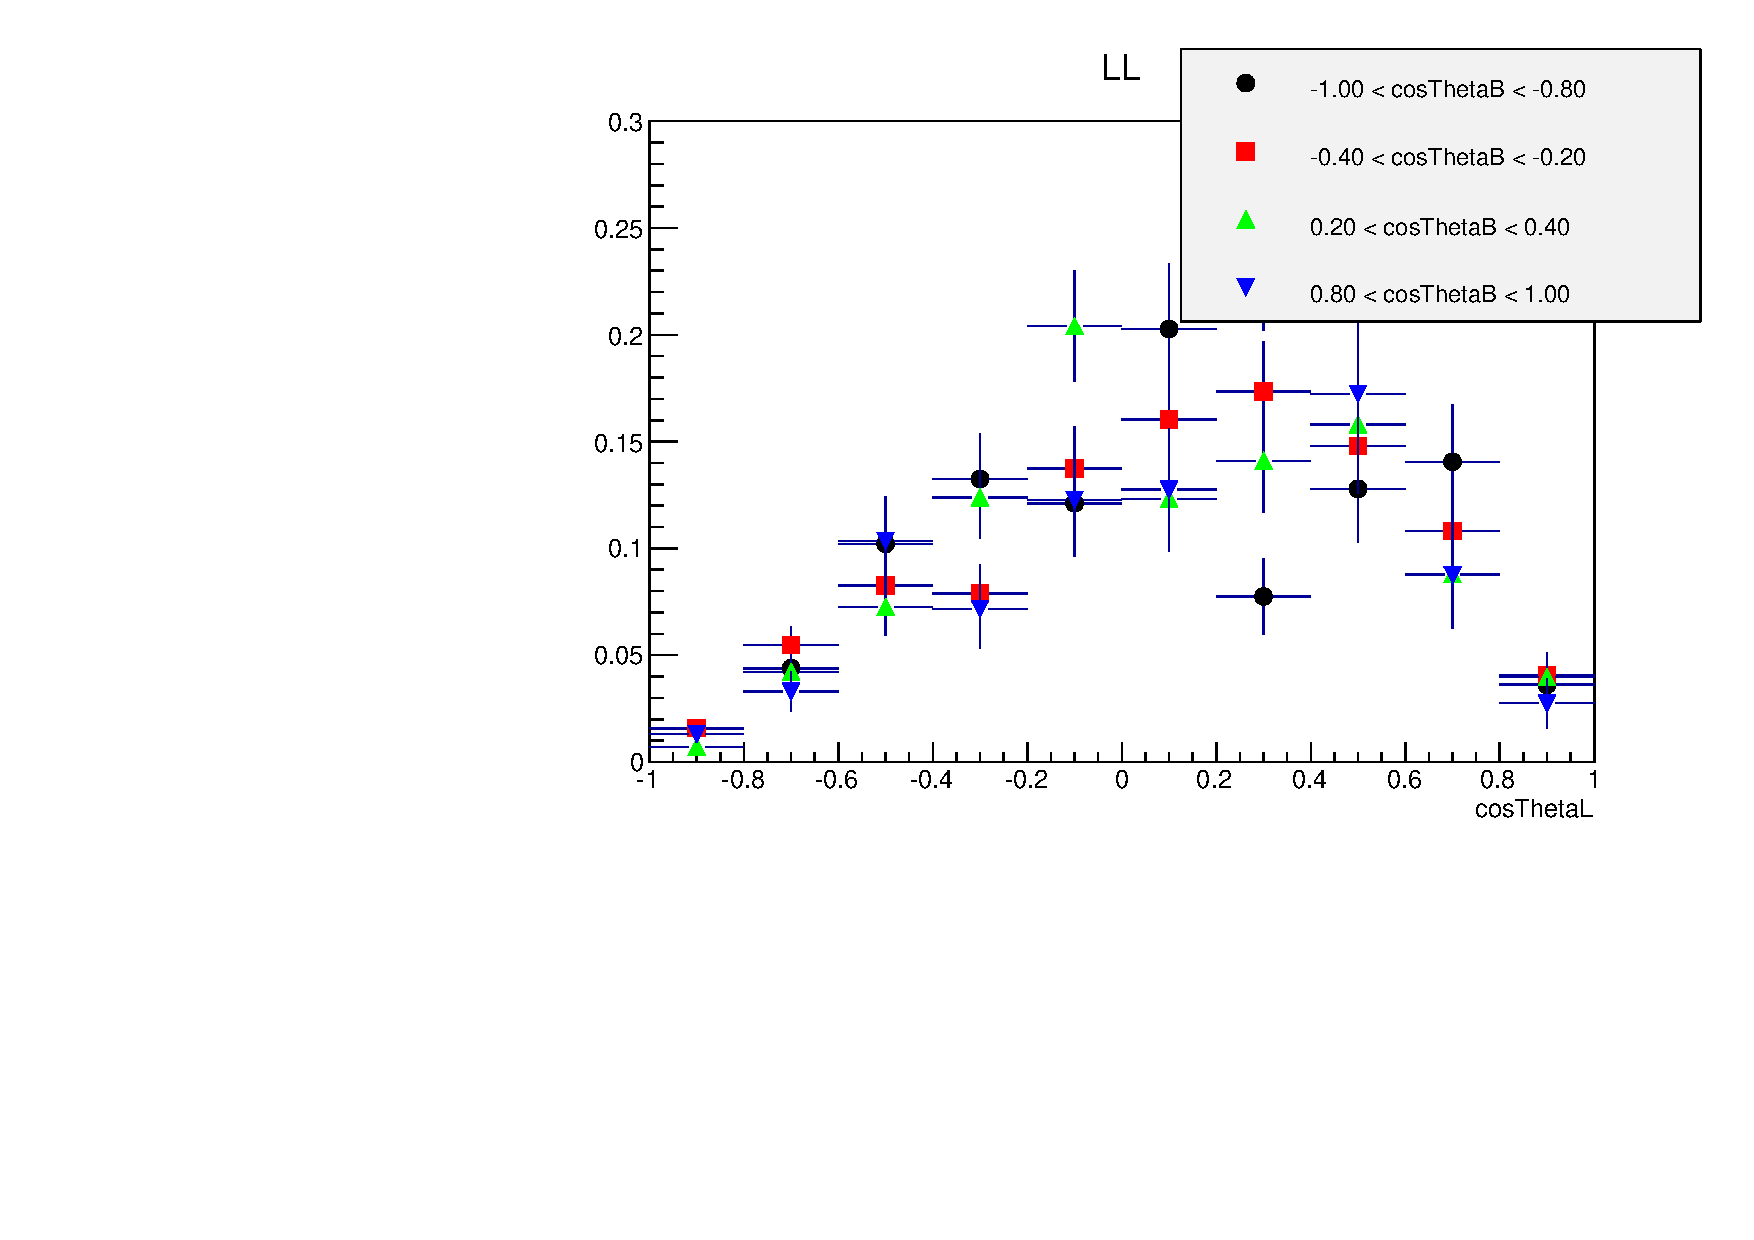
\includegraphics[width=0.45\textwidth]{Lmumu/figs/effs/LLeff_lowestq2.pdf}
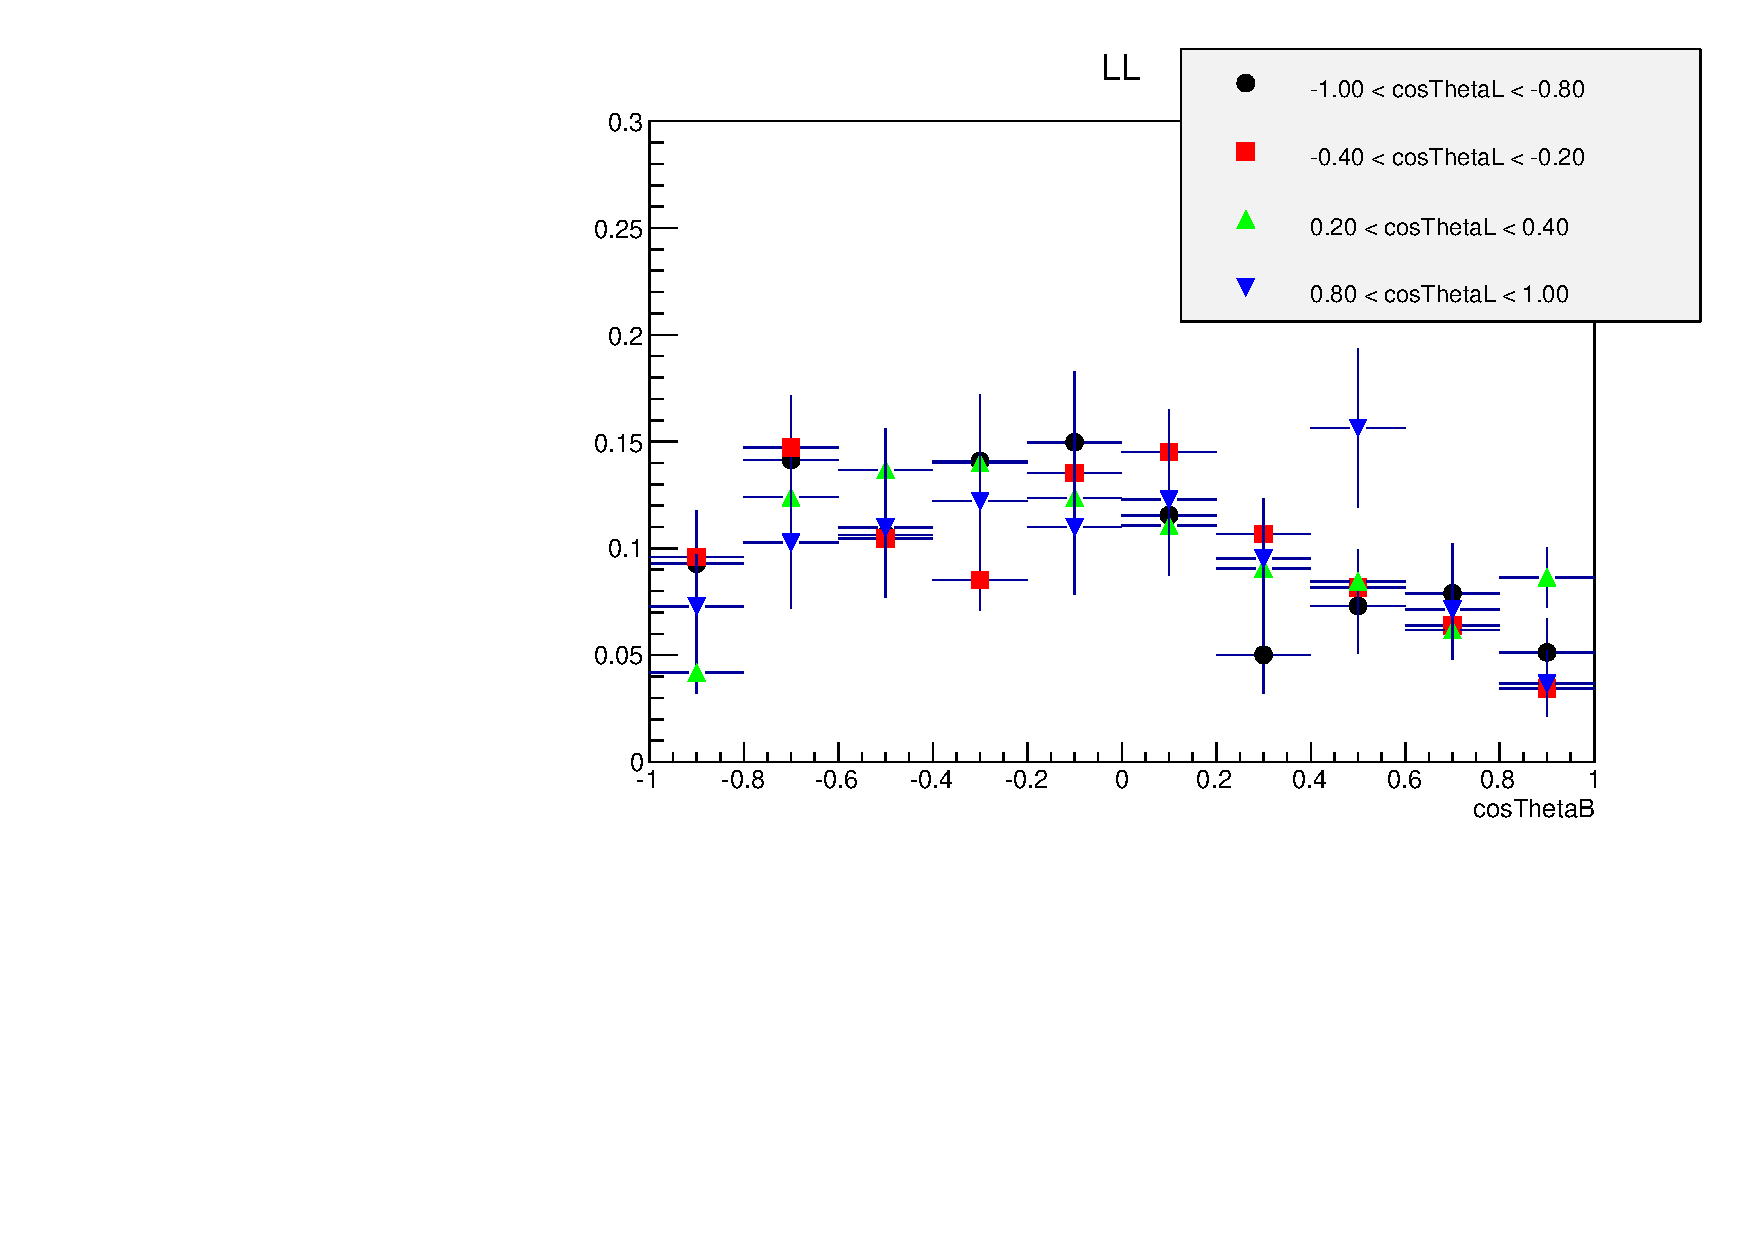
\includegraphics[width=0.45\textwidth]{Lmumu/figs/effs/LLBeff_lowestq2.pdf}
\caption{Angular acceptance as a function of $\cos\theta_\ell$ in bins of $\cos\theta_\Lambda$ (left) and viceversa (right). For long-long events in the lowest \qsq bin: $1.1 < q^2 < 3$}
\end{figure}



\begin{figure}[h!]
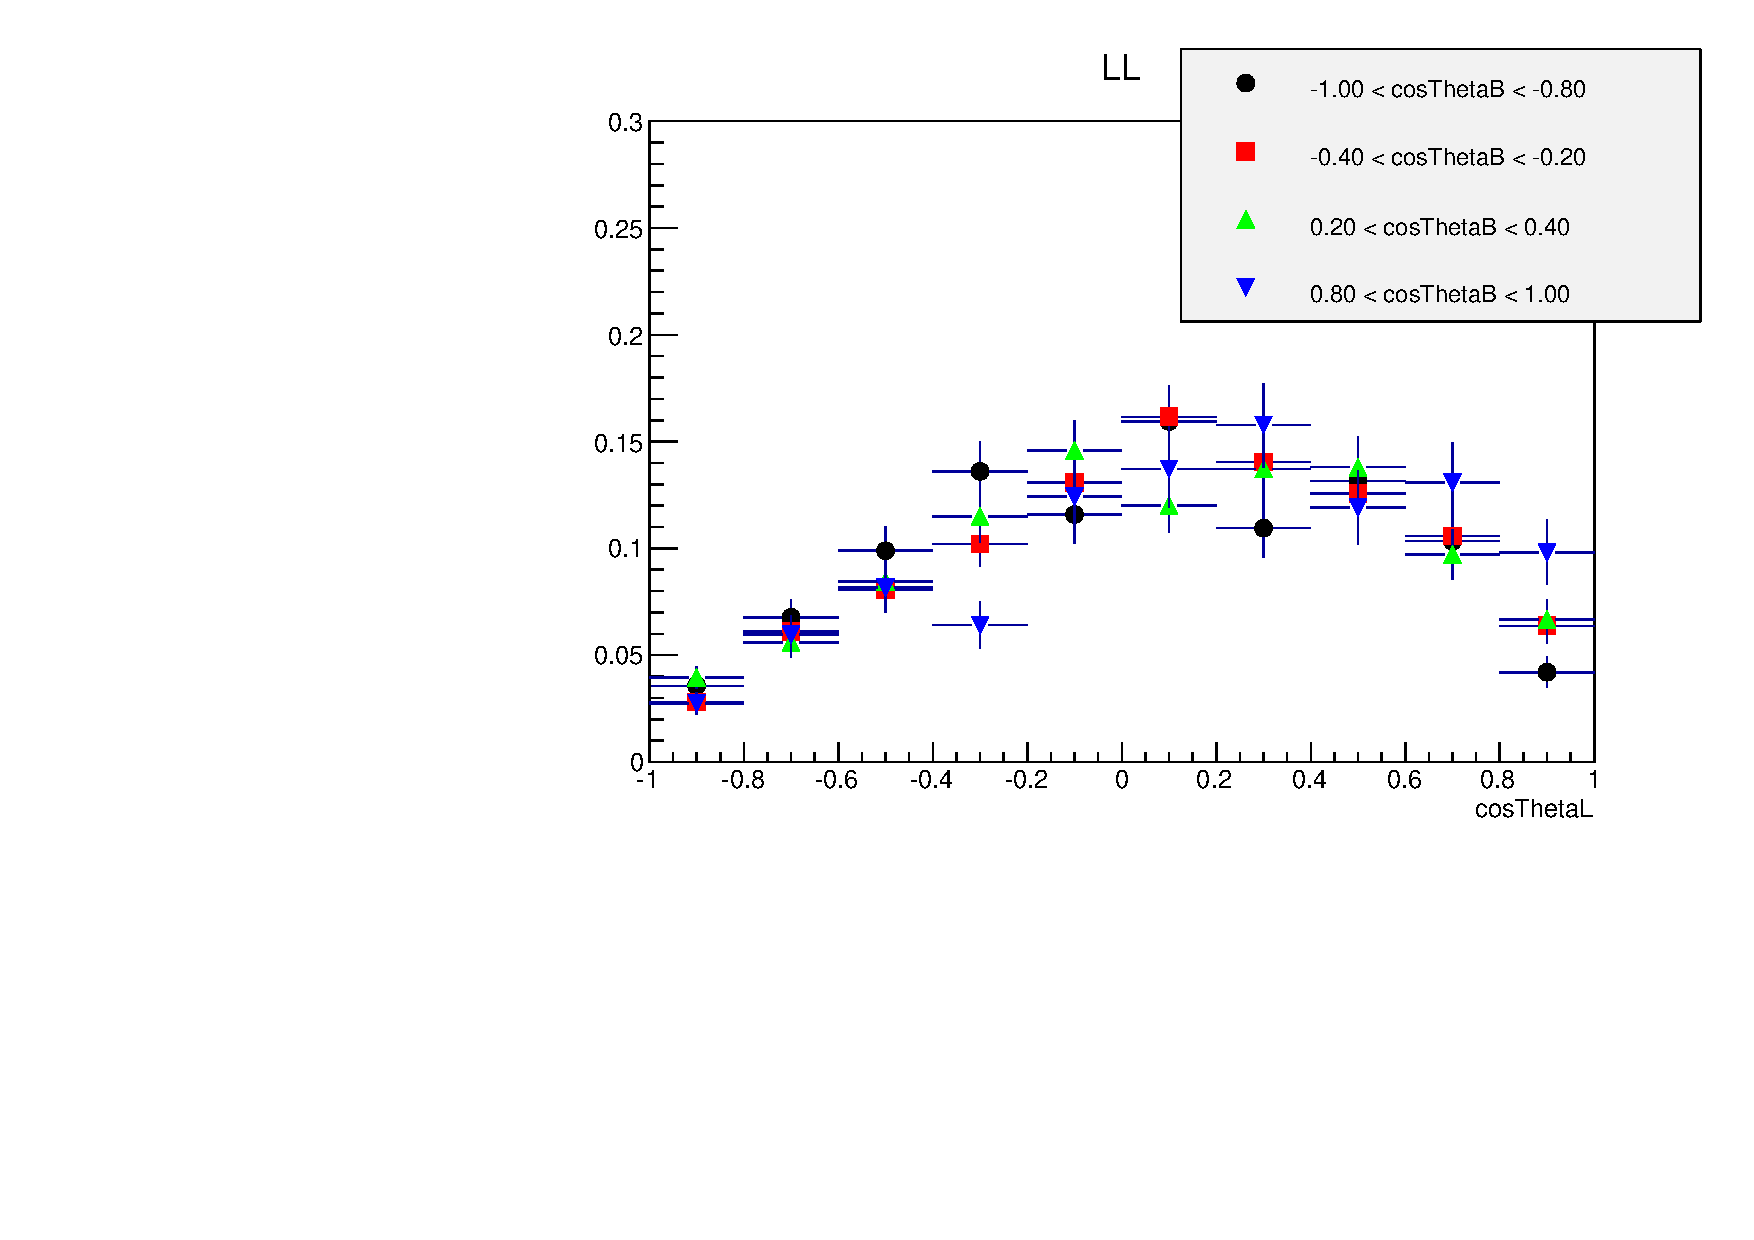
\includegraphics[width=0.45\textwidth]{Lmumu/figs/effs/LLeff_lowq2.pdf}
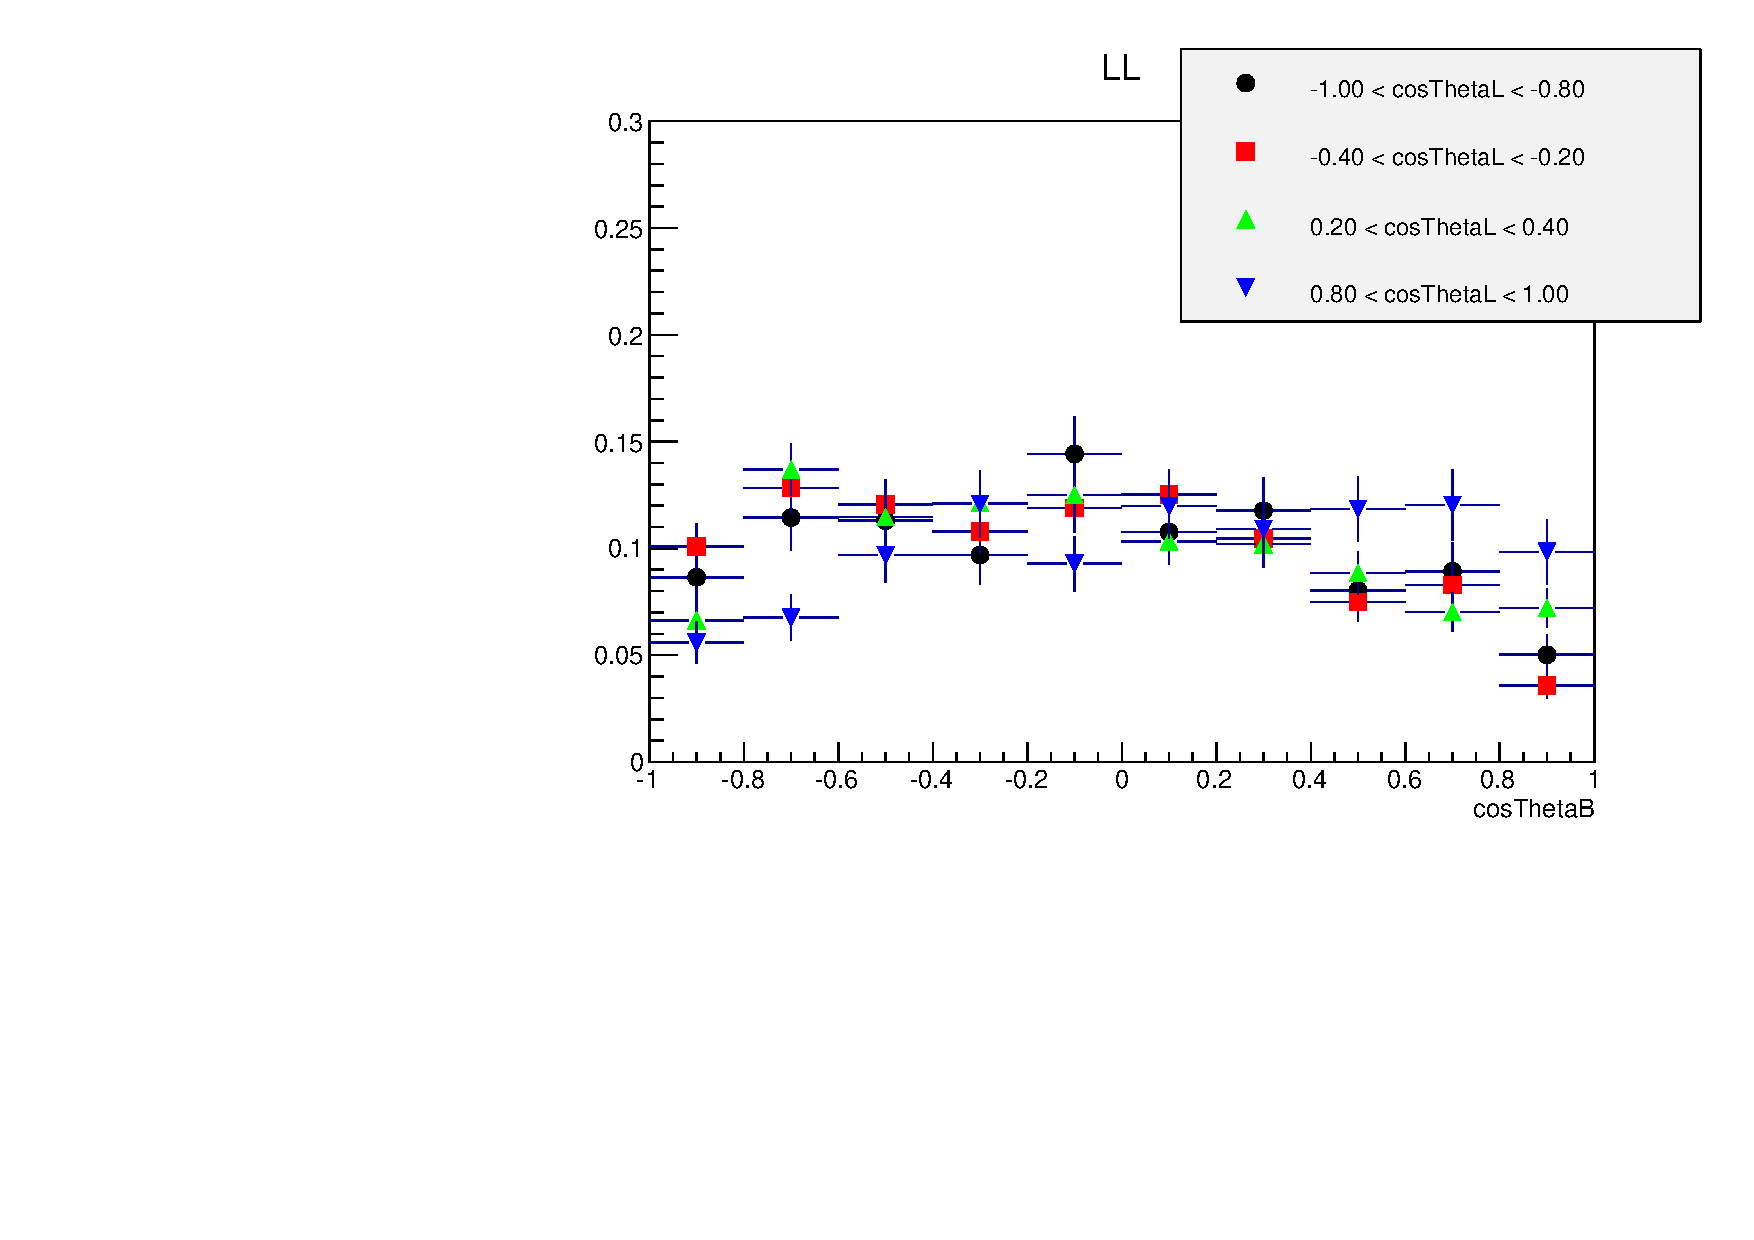
\includegraphics[width=0.45\textwidth]{Lmumu/figs/effs/LLBeff_lowq2.pdf}
\caption{Angular acceptance as a function of $\cos\theta_\ell$ in bins of $\cos\theta_\Lambda$ (left) and viceversa (right). For long-long events in the integrated low \qsq bin: $1.1 < q^2 < 6$}
\end{figure}



\begin{figure}[h!]
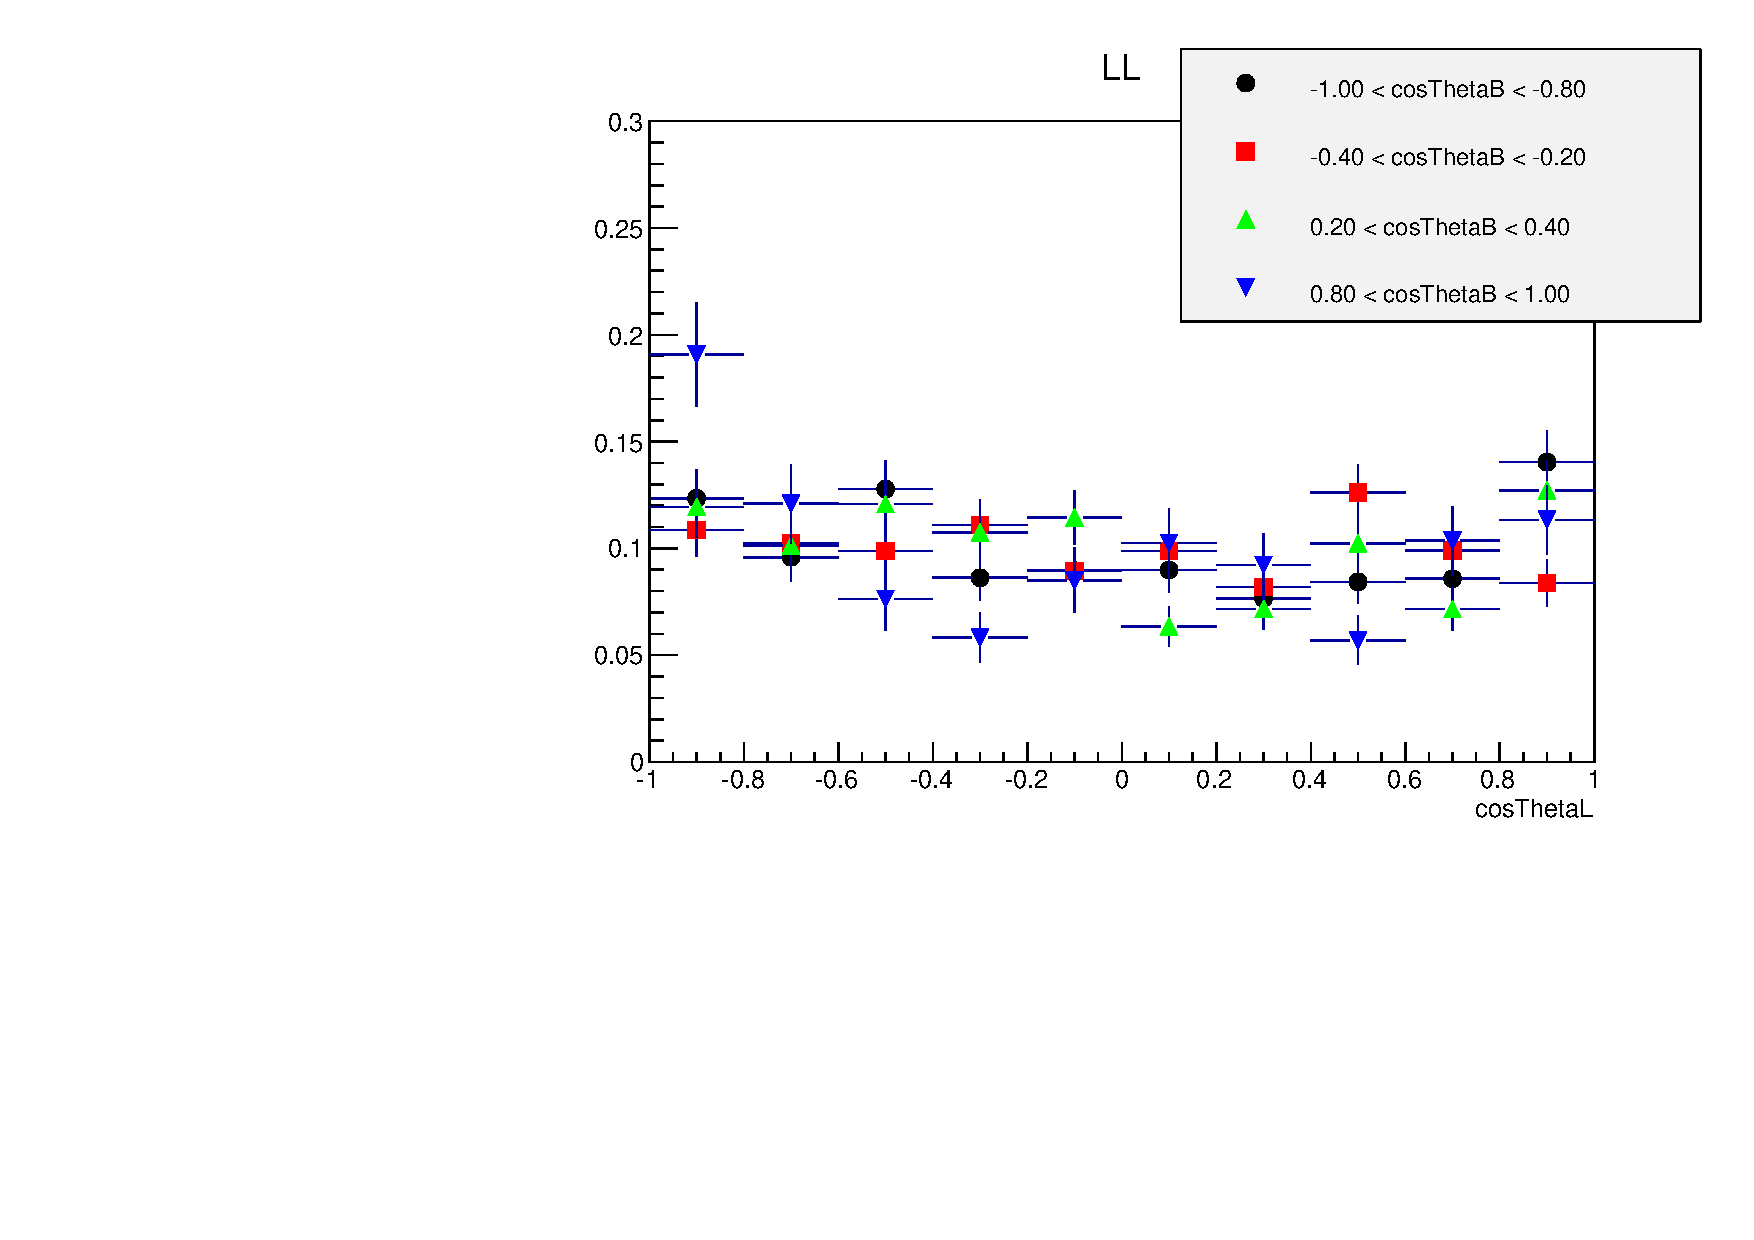
\includegraphics[width=0.45\textwidth]{Lmumu/figs/effs/LLeff_highq2.pdf}
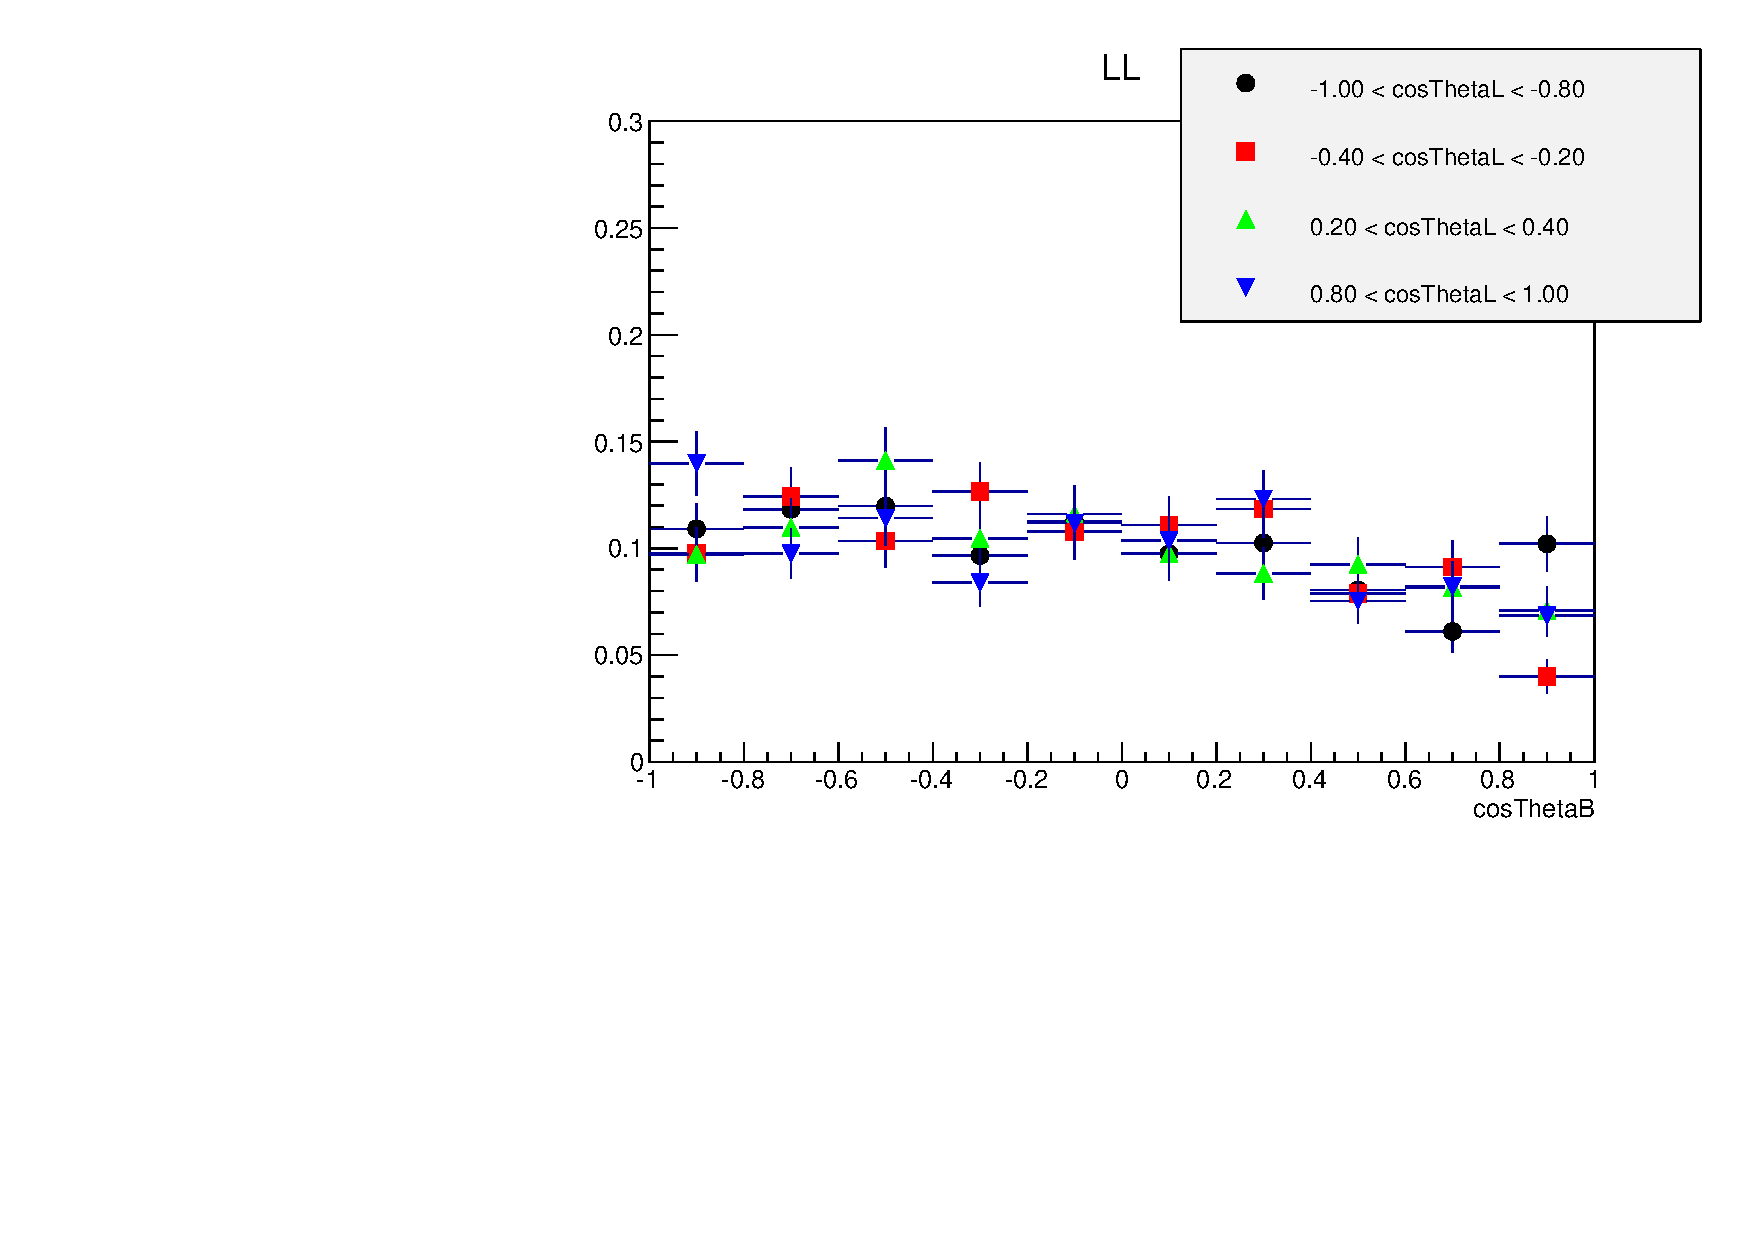
\includegraphics[width=0.45\textwidth]{Lmumu/figs/effs/LLBeff_highq2.pdf}
\caption{Angular acceptance as a function of $\cos\theta_\ell$ in bins of $\cos\theta_\Lambda$ (left) and viceversa (right). For long-long events in the integrated high \qsq bin: $15 < q^2 < 20$}
\end{figure}




\begin{figure}[h!]
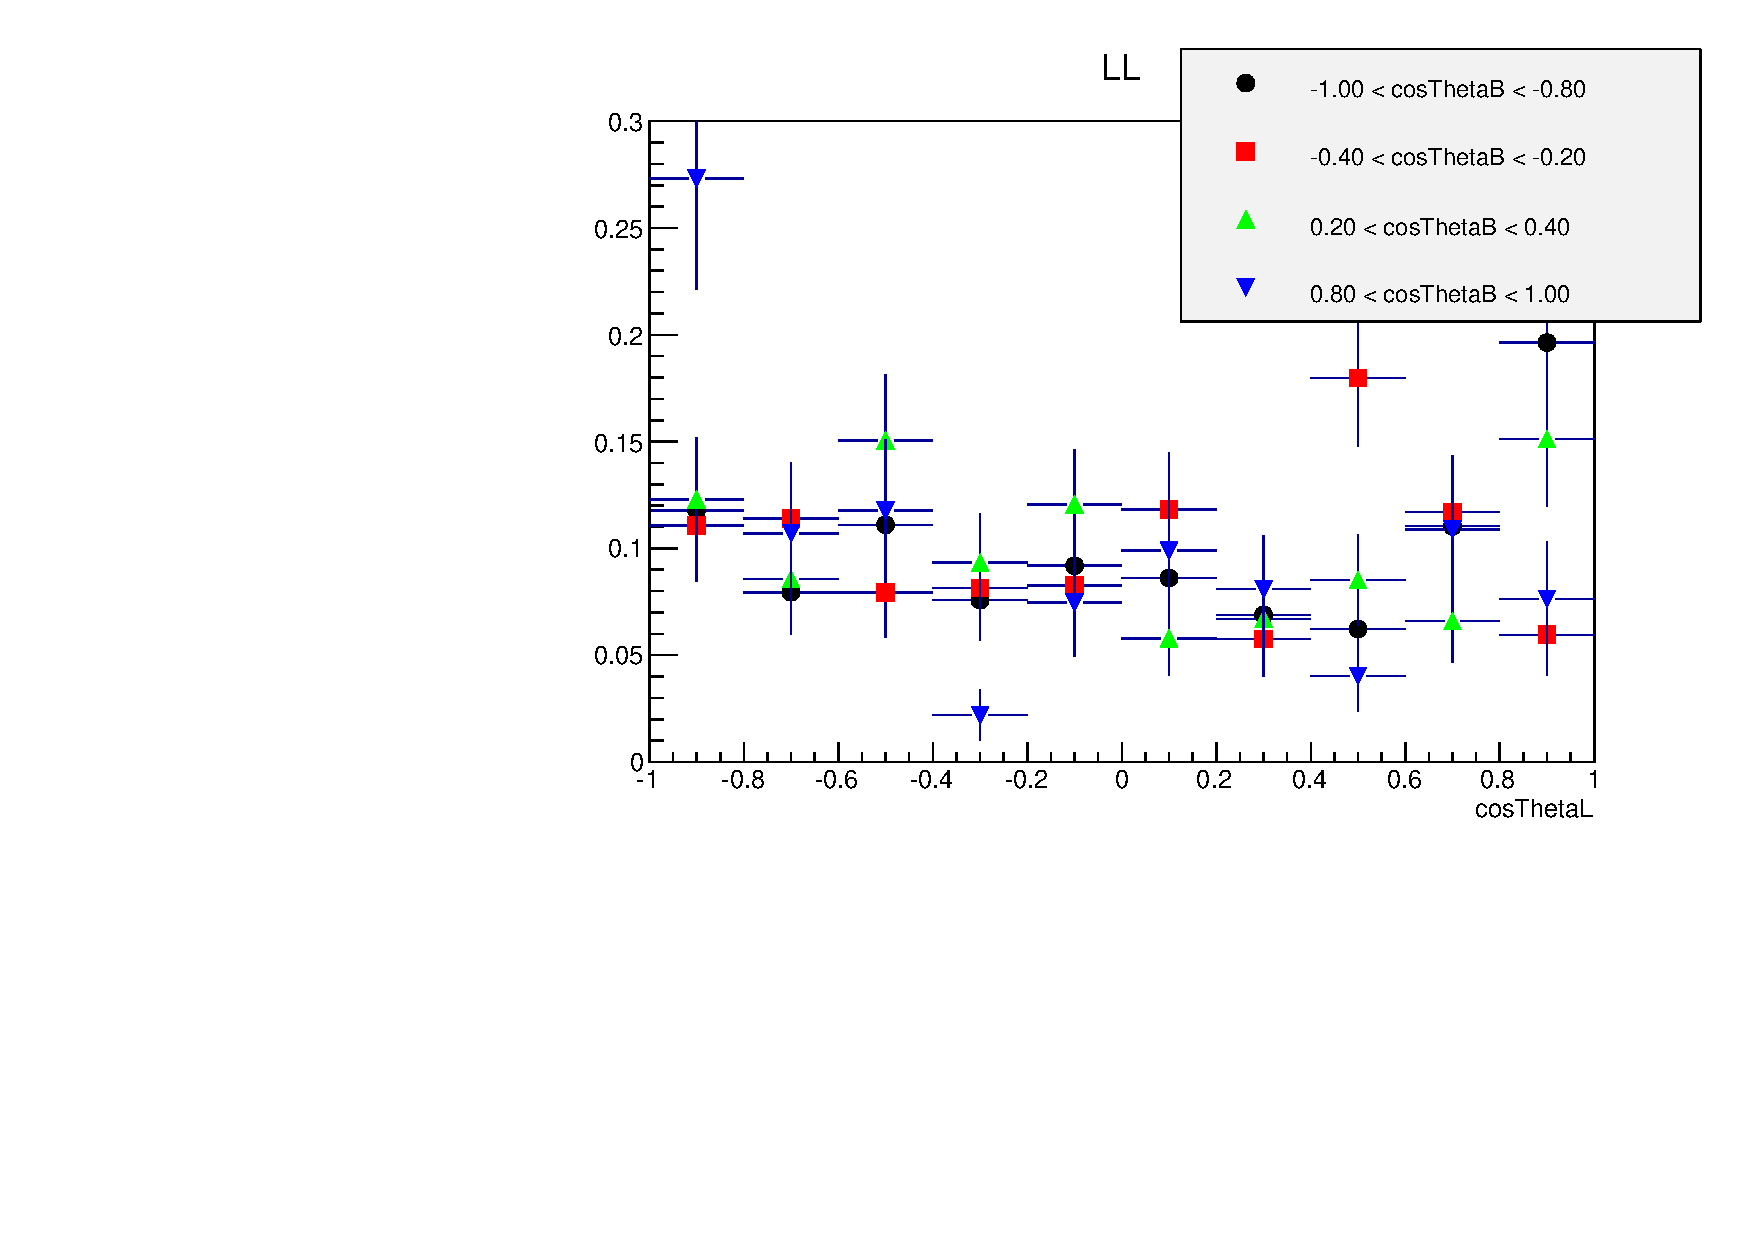
\includegraphics[width=0.45\textwidth]{Lmumu/figs/effs/LLeff_highestq2.pdf}
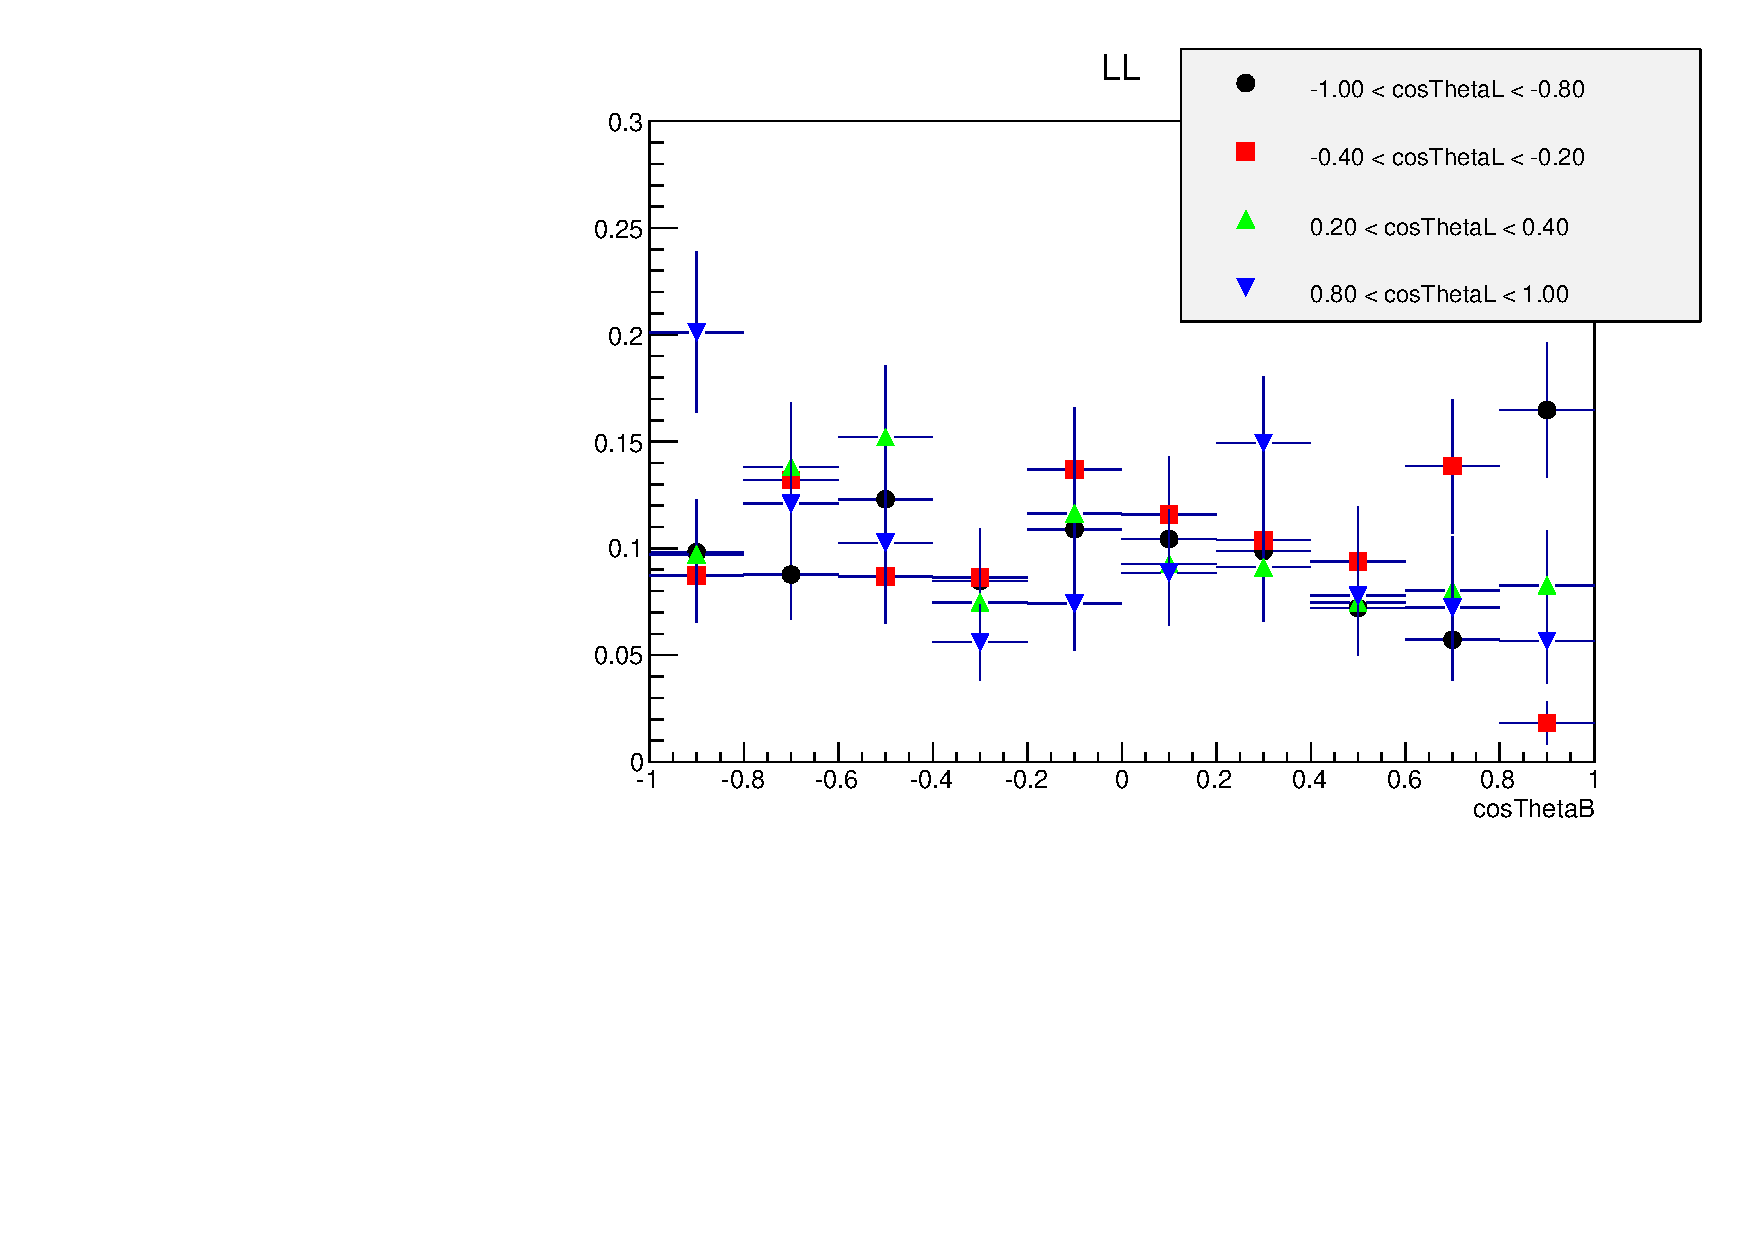
\includegraphics[width=0.45\textwidth]{Lmumu/figs/effs/LLBeff_highestq2.pdf}
\caption{Angular acceptance as a function of $\cos\theta_\ell$ in bins of $\cos\theta_\Lambda$ (left) and viceversa (right). For long-long events in the highest \qsq bin: $18 < q^2 < 20$}
\end{figure}



\begin{figure}[h!]
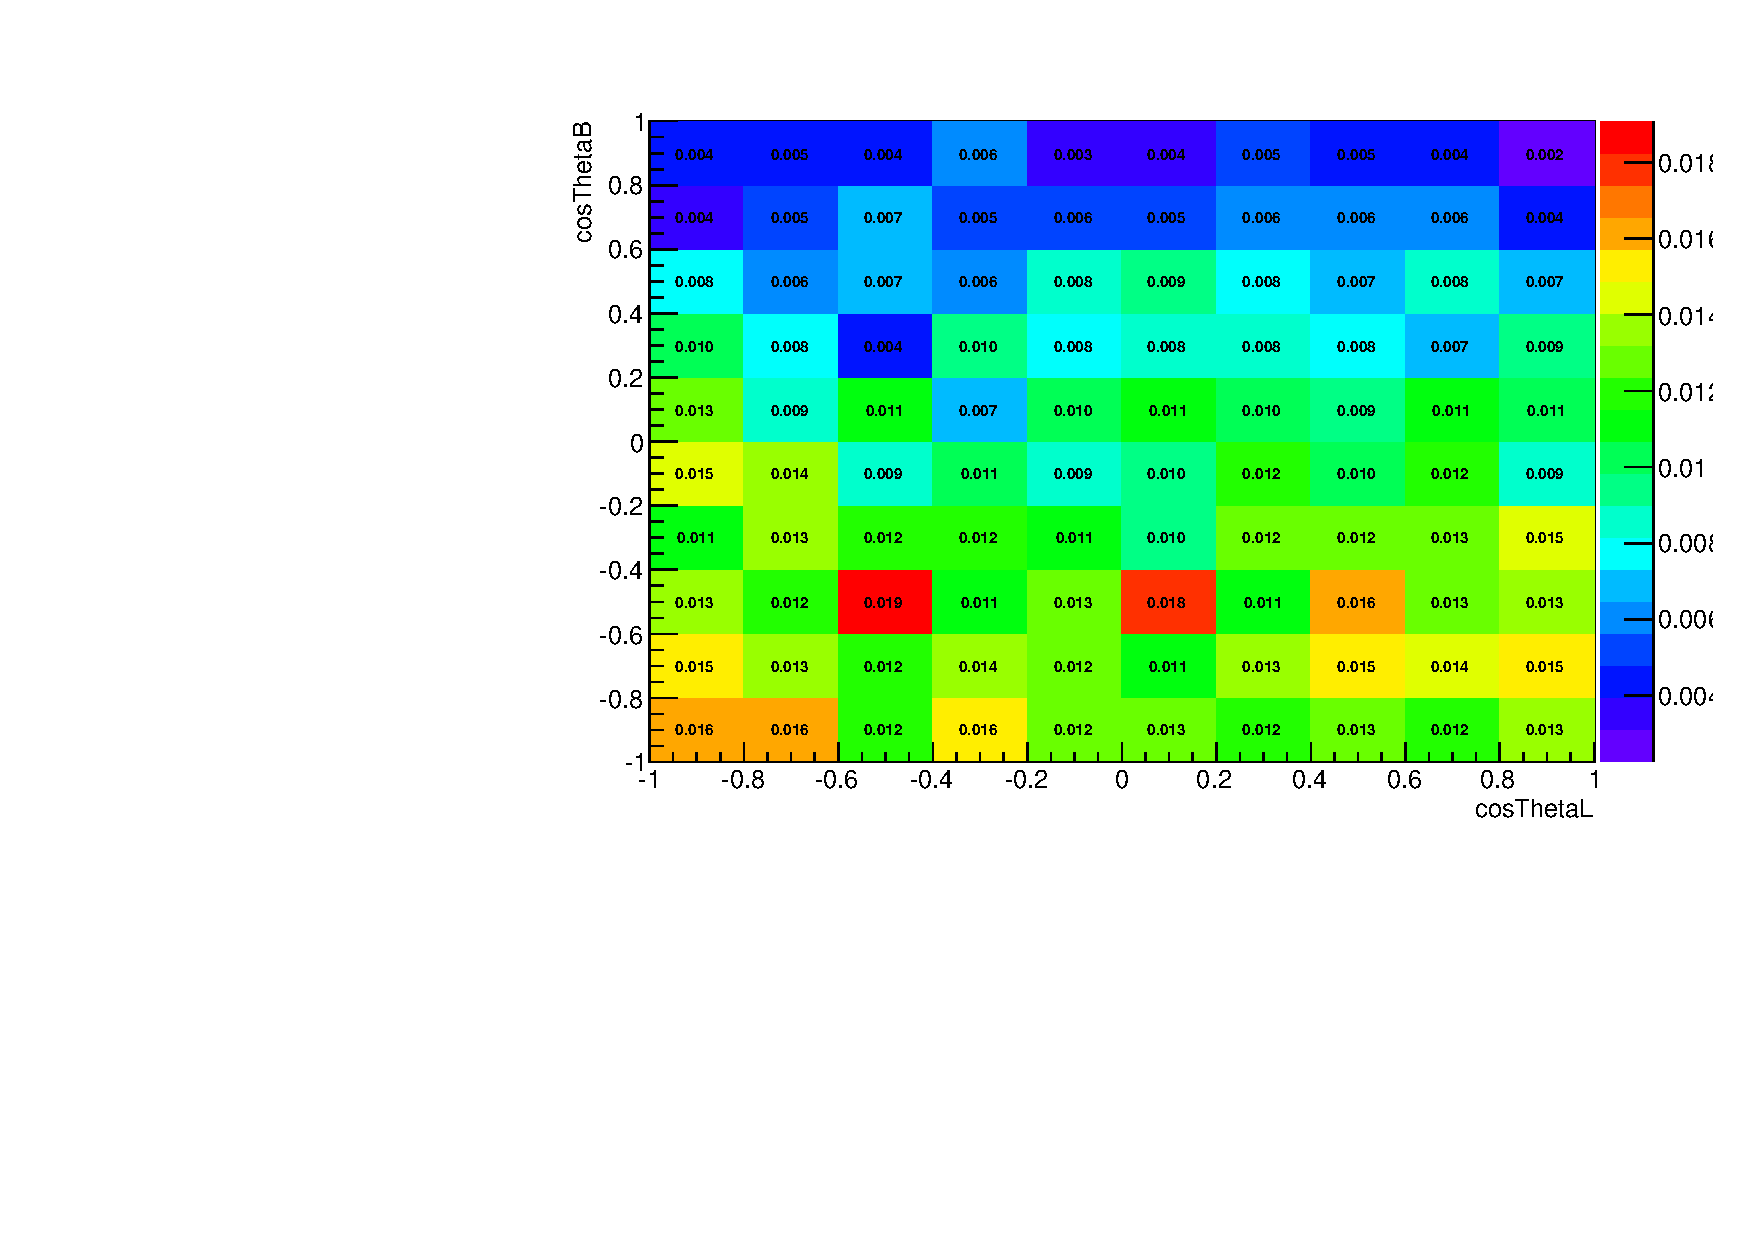
\includegraphics[width=0.9\textwidth]{Lmumu/figs/2Deff_upper_cosThetaB_vs_cosThetaL_DD.pdf}
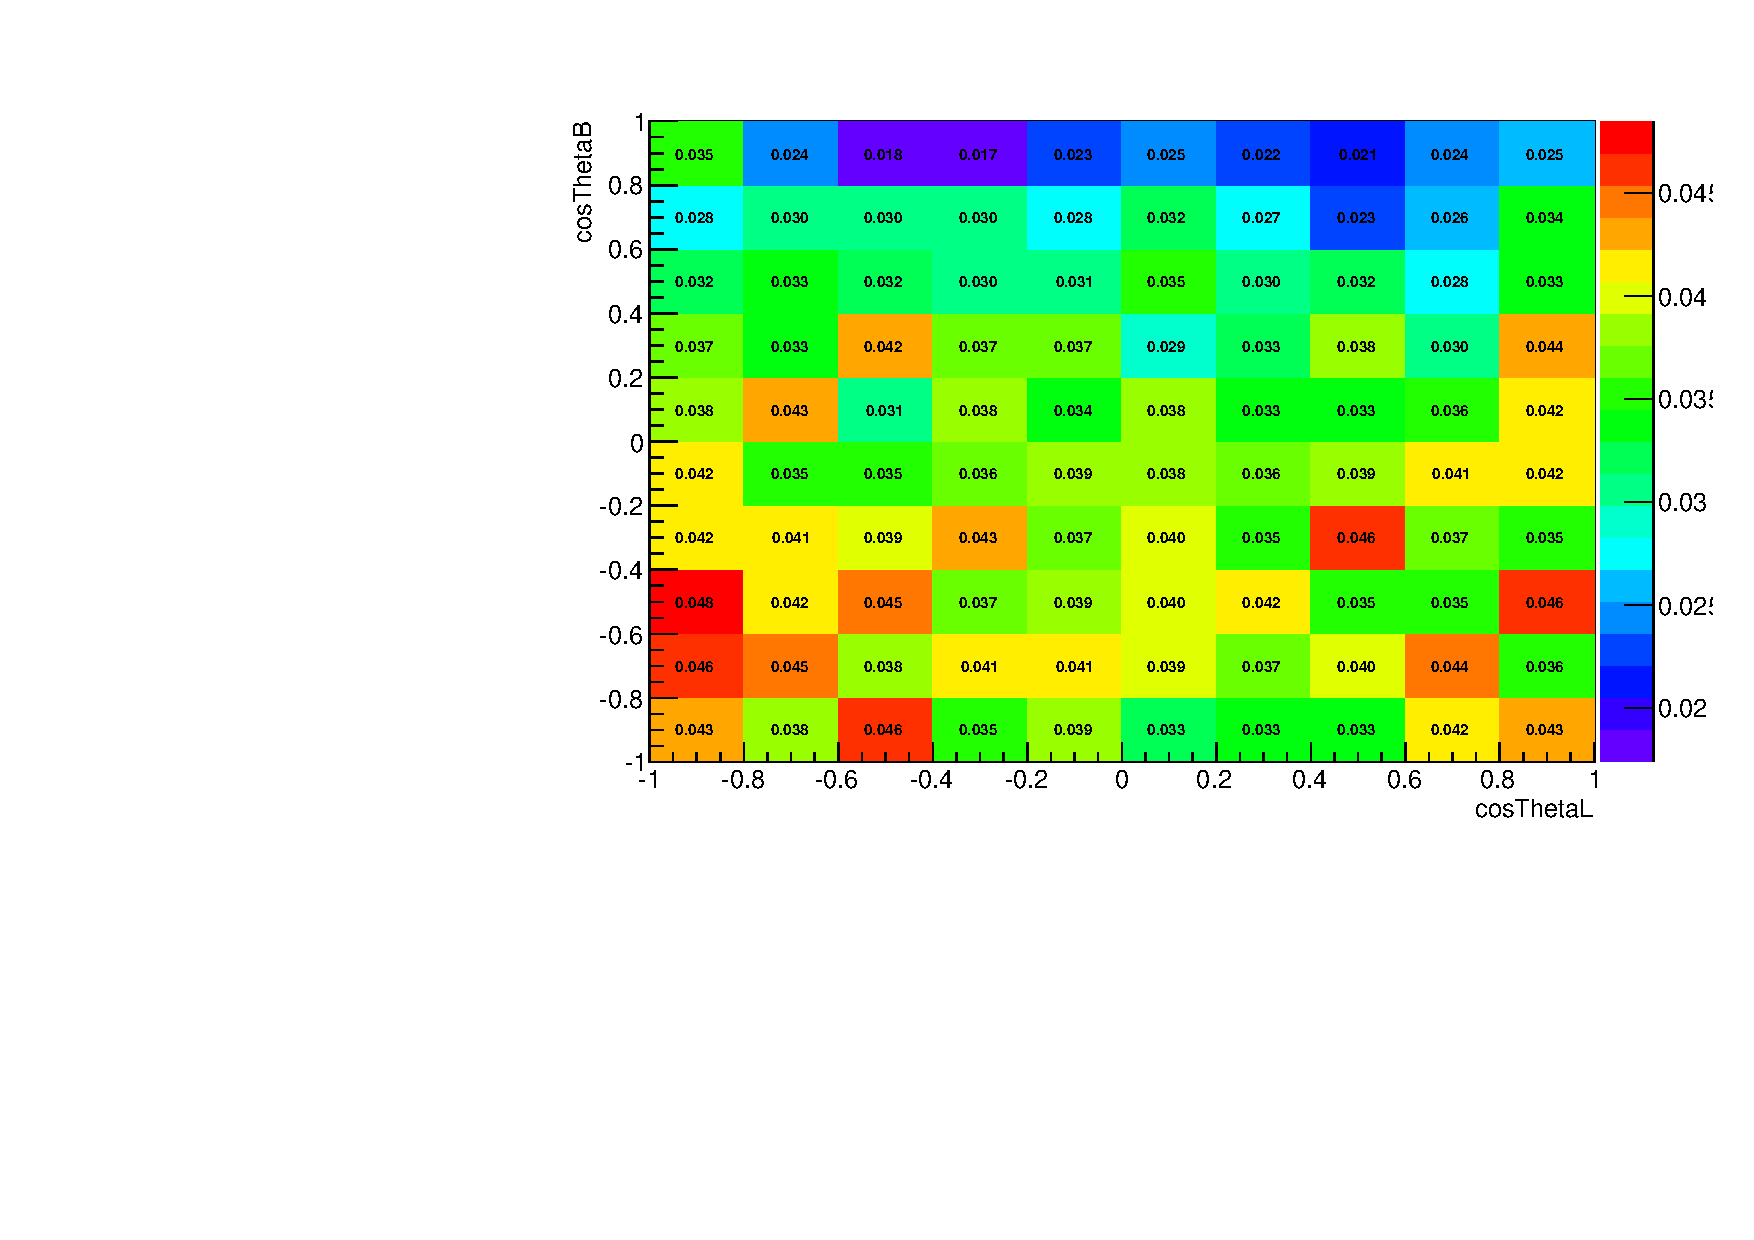
\includegraphics[width=0.9\textwidth]{Lmumu/figs/2Deff_upper_cosThetaB_vs_cosThetaL_LL.pdf}
\caption{Angular acceptance as a function of $\cos\theta_\ell$ and $\cos\theta_h$ for long (left) and
downstream (right) candidates, integrated over the full available \qsq range.}
\label{fig:2DcosThetaLandBeff}
\end{figure}

\clearpage
